% ==============================================================================
% Universidade Federal do Rio Grande do Norte
% Programa de Pós-Graduação em Engenharia Elétrica e de Computação
% Qualificação de mestrado
% Autor: Diogo Leite Rebouças <diogolr@gmail.com>
% ==============================================================================

\documentclass{beamer}

% Temas ========================================================================
\mode<presentation>
{
%\usetheme[blue,noshadow]{Trondheim}
%\usetheme[blue,minimal]{Trondheim}
\usetheme[blue,compress,numbers,nonav]{Trondheim}
%\usetheme[sand,compress,numbers,nonav,innovation]{Trondheim}
%\usetheme{default}

% Inner ........................................................................
%\useinnertheme{default}
%\useinnertheme{rounded}
%\useinnertheme{inmargin}
%\useinnertheme{rectangles}
\useinnertheme{circles}

% Outer ........................................................................
%\useoutertheme{default}
%\useoutertheme{infolines}
%\useoutertheme{miniframes}
%\useoutertheme{ntnu}
%\useoutertheme{shadow}
%\useoutertheme{sidebar}
%\useoutertheme{smoothbars}
%\useoutertheme{smoothtree}
%\useoutertheme{split}
%\useoutertheme{tree}

% Color ........................................................................
%\usecolortheme{albatross}
%\usecolortheme{beaver}
%\usecolortheme{beetle}
%\usecolortheme{crane}
%\usecolortheme{default}
%\usecolortheme{dolphin}
%\usecolortheme{dove}
%\usecolortheme{fly}
%\usecolortheme{lily}
%\usecolortheme{ntnublue}
%\usecolortheme{ntnuold}
%\usecolortheme{orchid}
%\usecolortheme{rose}
%\usecolortheme{seagull}
%\usecolortheme{seahorse}
%\usecolortheme{sidebartab}
%\usecolortheme{structure}
%\usecolortheme{whale}
%\usecolortheme{wolverine}
}

% Pacotes ======================================================================
% Pacotes Principais -----------------------------------------------------------
\usepackage[portuges,brazil]{babel}
\usepackage[utf8]{inputenc}

% Formatação de capítulos ------------------------------------------------------
%\usepackage[Sonny]{fncychap}
%\usepackage{fncychap}
\usepackage{capitulos}

% Figuras e Imagens ------------------------------------------------------------
\usepackage{graphicx}
% Figuras lado a lado
\usepackage{epsfig}
\usepackage{subfigure}

% Tikz
\usepackage{tikz}
\usepackage{pgfplots}
\pgfplotsset{compat=1.3}
\usepackage{tikz-timing}[2009/05/15]

% Utilizar H para inserir as imagens REALMENTE onde eu desejo
\usepackage{float}

% Fontes -----------------------------------------------------------------------
\usepackage[T1]{fontenc}
\usepackage{pslatex}

% Simbolos ---------------------------------------------------------------------
\usepackage{textcomp}

% Tabelas ----------------------------------------------------------------------
%\usepackage{multicol}
\usepackage{multirow}
% Colorir a tabela
\usepackage{colortbl}
% Tabelas com colunas de largura auto ajustável
\usepackage{tabularx}
% Notas de rodapé em tabelas (Pode-se usar o ambiente longtable também -
% Pesquisar exemplo com longtable)
\usepackage{threeparttable}

% Glossário --------------------------------------------------------------------
\usepackage[portuguese,noprefix]{nomencl}
\usepackage{makeglo}

% Outros pacotes ---------------------------------------------------------------
\usepackage{noitemsep}

% Comentários em bloco
\usepackage{verbatim}

% Hiperlinks
\usepackage{hyperref}

% Orientação de página
\usepackage{lscape}

% utilitários matemáticos
\usepackage{amsmath}
\usepackage{icomma}

% Referências ------------------------------------------------------------------
\usepackage[abbr]{harvard}	% As chamadas são sempre abreviadas
\harvardparenthesis{square}	% Colchetes nas chamadas
\harvardyearparenthesis{round}	% Parêntesis nos anos das referências
\renewcommand{\harvardand}{e}	% Substituir "&" por "e" nas referências


% Comandos =====================================================================
% Comandos gerais --------------------------------------------------------------
\newcommand{\titulo}{Utilização de redes neurais artificiais para detecção e
diagnóstico de falhas}
\newcommand{\autor}{Diogo Leite Rebouças}
\newcommand{\emailautor}{\tt diogolr@dca.ufrn.br}
\newcommand{\orientador}{Fábio Meneghetti Ugulino de Araújo}
%\newcommand{\coorientador}{André Laurindo Maitelli}
\newcommand{\diaaprovacao}{21}
% Mês com inicial maiúscula (capa, folha de rosto)
\newcommand{\Mesaprovacao}{Junho}
% Mês com inicial minúscula (folha de assinaturas)
\newcommand{\mesaprovacao}{junho}
\newcommand{\anoaprovacao}{2011}
\let\Anoaprovacao\anoaprovacao
\newcommand{\dataaprovacao}{\diaaprovacao\ de \mesaprovacao\ de \anoaprovacao}
% Tipo de documento
\newcommand{\documento}{Defesa de Dissertação}
% Nome da ufrn
\newcommand{\ufrn}{Universidade Federal do Rio Grande do Norte}
% Nome do programa de pós-graduação
\newcommand{\ppgeec}{Programa de Pós-Graduação em Engenharia Elétrica e de
                     Computação}

% Configuração da fonte
%\renewcommand{\familydefault}{\sfdefault}

% Comandos matemáticos ---------------------------------------------------------
% Implicação em fórmulas
\newcommand{\implica}{$\quad\Rightarrow\quad$} %Meio de linha
\newcommand{\implicafim}{$\quad\Rightarrow$}   %Fim de linha
\newcommand{\tende}{$\rightarrow$}

% Fração com parenteses
\newcommand{\pfrac}[2]{\parent{\frac{#1}{#2}}}

% Transformada de Laplace e transformada Z
\newcommand{\lapl}{\pounds}
\newcommand{\transfz}{\mathcal{Z}}

% Sequências
\newcommand{\sequencia}[4]{$#1_{#2}$, $#1_{#3}$, \ldots, $#1_{#4}$}

% Outros ----------------------------------------------------------------------
\newcommand{\chave}[1]{\left\{#1\right\}}
\newcommand{\colchete}[1]{\left[#1\right]}
\newcommand{\parent}[1]{\left(#1\right)}

\newcommand{\rhoagua}{\rho_{\tiny \text{\tiny H}_2\text{\tiny O}}}
\newcommand{\reg}{\textsuperscript{\textregistered}}

\let\D\displaystyle

\newtheorem{teorema}{Teorema}
\newtheorem{exemplo}{Exemplo}
\newtheorem{definicao}{Definição}
\newtheorem{lema}{Lema}
\newcommand{\defin}[1]{\begin{definicao}#1\end{definicao}}

% Imagens exportadas pelo gnuplot ----------------------------------------------
\graphicspath{{imgs/resultados/eps/}}

% Hyperref ---------------------------------------------------------------------
\hypersetup{
    bookmarks=true,         % show bookmarks bar?
    unicode=false,          % non-Latin characters in Acrobat’s bookmarks
    pdftoolbar=true,        % show Acrobat’s toolbar?
    pdfmenubar=true,        % show Acrobat’s menu?
    pdffitwindow=false,     % window fit to page when opened
    pdfstartview={FitH},    % fits the width of the page to the window
    pdftitle={\titulo},     % title
    pdfauthor={\autor},     % author
    pdfsubject={mestrado},  % subject of the document
    pdfcreator={\autor},    % creator of the document
    pdfproducer={\autor},   % producer of the document
    pdfkeywords={Controle}, % list of keywords
    pdfnewwindow=true,      % links in new window
    colorlinks=false,       % false: boxed links; true: colored links
    linkcolor=black,        % color of internal links
    citecolor=black,        % color of links to bibliography
    filecolor=black,        % color of file links
    urlcolor=black          % color of external links
}

% Outros -----------------------------------------------------------------------
% Transparência dos tópicos
\setbeamercovered{transparent}

% Sumário entre as seções
\AtBeginSection[]
{
\begin{frame}
\frametitle{Sumário}
    \footnotesize
    \begin{columns}
        \column{0.45\textwidth}
            \tableofcontents[sections=1,currentsection]
            \vspace{0.25cm}
            \tableofcontents[sections=2,currentsection]
            \vspace{0.25cm}
            \tableofcontents[sections=3,currentsection]
        \column{0.45\textwidth}
            \tableofcontents[sections=4,currentsection]
            \vspace{0.25cm}
            \tableofcontents[sections=5,currentsection]
            \vspace{0.25cm}
            \tableofcontents[sections=6,currentsection]
            \vspace{0.25cm}
            \tableofcontents[sections=7,currentsection]
    \end{columns}
\end{frame}
}

% Sumário entre as subseções
%\AtBeginSubsection[]
%{
%\begin{frame}
%\frametitle{Sumário}
%\tableofcontents[currentsection,currentsubsection]
%\end{frame}
%}


% Configuração da página inicial ===============================================
\title[Exame de Qualificação de Mestrado]
{
    Exame de Qualificação de Mestrado
}
\subtitle{\small\titulo}
\author[Diogo Leite Rebouças]
{
    \autor\\
    \emailautor
}
\institute
{
    Universidade Federal do Rio Grande do Norte\\
    Programa de Pós-Graduação em Engenharia Elétrica e Computação
}
%\date{\today}
\date{\dataaprovacao}
\pgfdeclareimage[width=3cm,interpolate=true]
                {ntnulogotext}{imgs/outras/eps/ufrn_trad}

% Inicio do documento ==========================================================
\begin{document}

\maketitle
%\compressedtitle

% Logo somente após a capa
\logo{
\includegraphics[width=2cm]{imgs/outras/eps/ufrn_trad}}

% Sumário ......................................................................
\begin{frame}
    \frametitle{Sumário}
    \footnotesize
    \begin{columns}
        \column{0.45\textwidth}
            \tableofcontents[sections=1]
            \vspace{0.25cm}
            \tableofcontents[sections=2]
            \vspace{0.25cm}
            \tableofcontents[sections=3]
        \column{0.45\textwidth}
            \tableofcontents[sections=4]
            \vspace{0.25cm}
            \tableofcontents[sections=5]
            \vspace{0.25cm}
            \tableofcontents[sections=6]
    \end{columns}
\end{frame}

% Introdução ...................................................................
\section{Introdução}

% TODO verificar necessidade de adicionar na dissertação
\begin{comment}
% ------------------------------------------------------------------------------
\subsection{Aspectos históricos}
\begin{frame}
    \frametitle{Aspectos históricos}
    História dos sistemas de controle \implica 300 a.C. a 250 a.C. \implica
    primeiras boias flutuadoras e o relógio de água de Ktesíbios

    \vspace{0.25cm}

    Controle automático \implica Após a revolução industrial (segunda metade do
    século XVIII)

\begin{figure}[htb]
\centering
    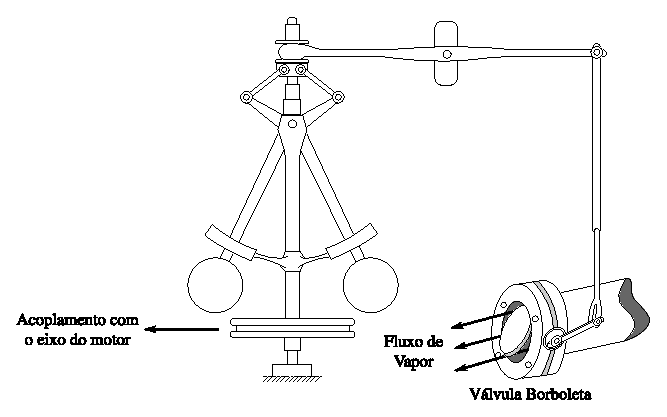
\includegraphics[width=0.65\textwidth]{imgs/introducao/eps/regulador_esferas}
\end{figure}

\end{frame}

\begin{frame}
    \frametitle{Aspectos históricos}

    Introdução desse assunto na indústria se deu durante a 2\textordfeminine\
    guerra \implica necessidade em se projetar e construir, por exemplo:

\begin{itemize}
    \item Pilotos automáticos para aeronaves
    \item Sistemas de posicionamento de armas
    \item Sistemas de controle para antenas e radares
\end{itemize}

    Ajustar os ganhos dos controladores \implica tentativa e erro

    \vspace{0.25cm}

    Publicação do artigo de Ziegler e Nichols (1942) \implica Disseminação dos
    controladores PID nas indústrias
\end{frame}
\end{comment}

% ------------------------------------------------------------------------------
\subsection{Introdução da automação na indústria}
\begin{frame}
    \frametitle{Introdução da automação na indústria}

    Com o surgimento dos CLPs e a popularização do controle automático, foco:

\begin{itemize}
    \item Desempenho dos processos
    \item Qualidade dos produtos 
    \item Independência de funcionamento da planta para com os operadores
          humanos
\end{itemize}

    Evolução \implica processos divididos em várias camadas de finalidades
    específicas:

% TODO retirar ao adicionar figuras dos slides seguintes
\begin{itemize}
    \item Controle (Inferior)
    \item Supervisão (Intermediário)
    \item Logística/Gerenciamento (Superior)
\end{itemize}
    
\end{frame}

% TODO adicionar na dissertação
\begin{comment}
\begin{frame}
    \frametitle{Introdução da automação na indústria}

\begin{figure}[htb]
\centering
    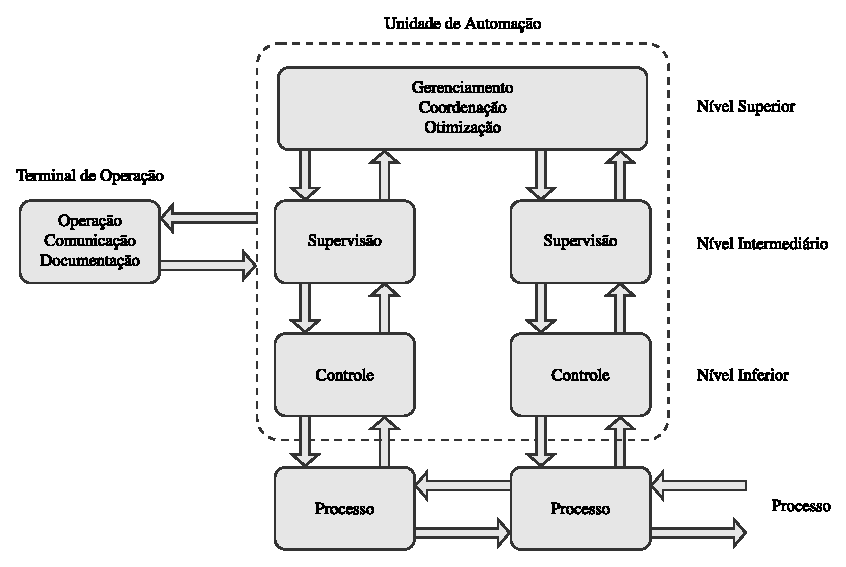
\includegraphics[width=0.9\textwidth]{imgs/introducao/eps/esquema_automacao}
\end{figure}
\end{frame}

\begin{frame}
    \frametitle{Introdução da automação na indústria}

\begin{figure}[htb]
\centering
    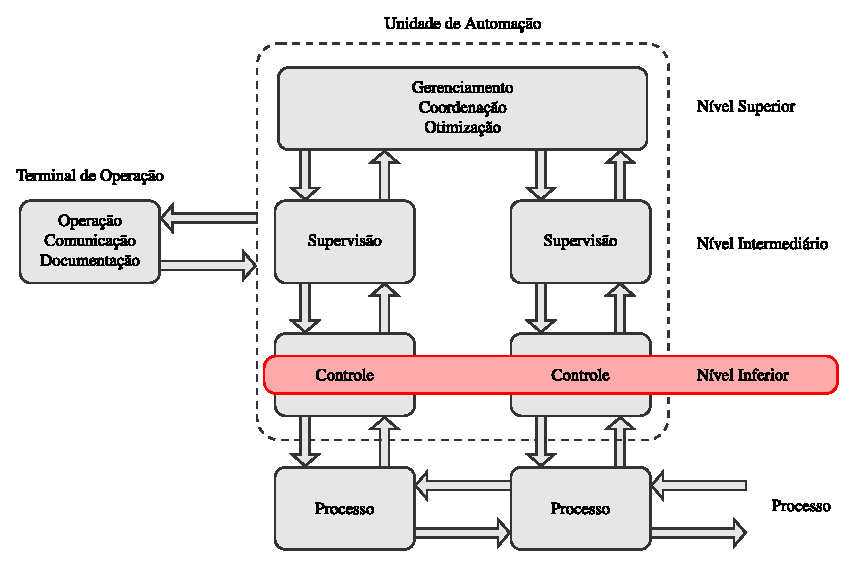
\includegraphics[width=0.9\textwidth]
    {imgs/introducao/eps/esquema_automacao_inf}
\end{figure}
\end{frame}

\begin{frame}
    \frametitle{Introdução da automação na indústria}

\begin{figure}[htb]
\centering
    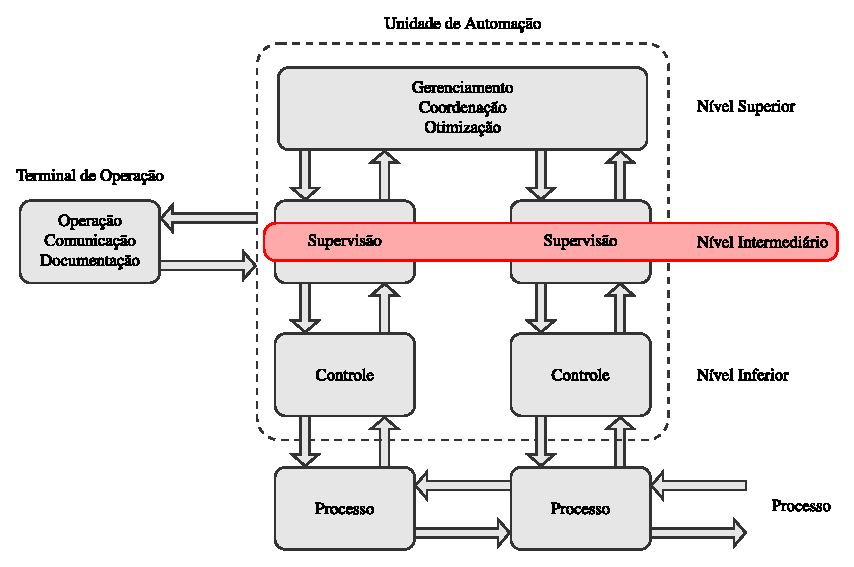
\includegraphics[width=0.9\textwidth]
    {imgs/introducao/eps/esquema_automacao_int}
\end{figure}
\end{frame}

\begin{frame}
    \frametitle{Introdução da automação na indústria}

\begin{figure}[htb]
\centering
    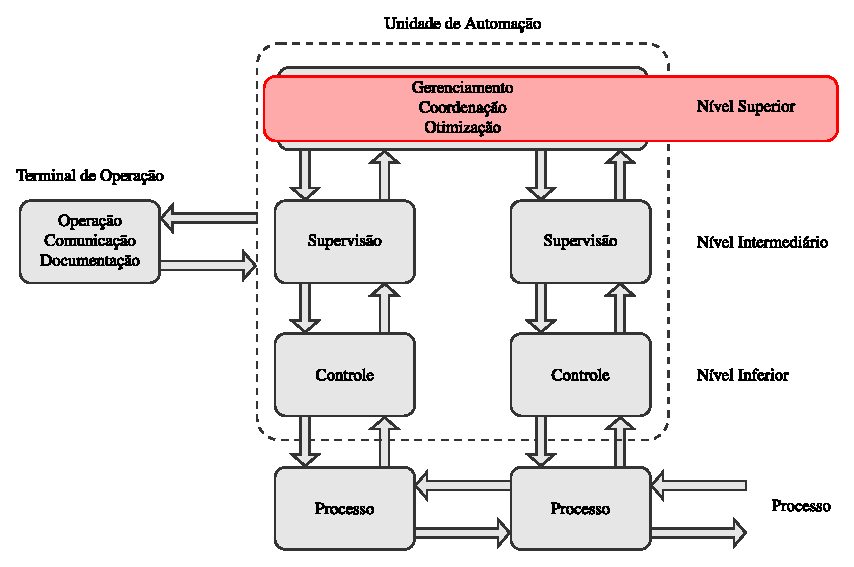
\includegraphics[width=0.9\textwidth]
    {imgs/introducao/eps/esquema_automacao_sup}
\end{figure}
\end{frame}
\end{comment}

\begin{frame}
    \frametitle{Introdução da automação na indústria}

    Eficiência das estratégias de controle aumenta (nível inferior):

\begin{itemize}
    \item Operadores são retirados do processo
    \item Operadores não se limitam a controlar o processo e mudar referências
          \implica realizam atividade de supervisão (contato direto)
\end{itemize}

    Deve-se melhorar estratégias de supervisão (nível intermediário)

\end{frame}

% ------------------------------------------------------------------------------
\subsection{Sistemas de supervisão}
\begin{frame}
    \frametitle{Sistemas de supervisão}

    Surgimento dos primeiros sistemas de supervisão:

\begin{itemize}
    \item Verificavam limites de determinadas variáveis
    \item Se o limite fosse ultrapassado \implica alarme para o operador
    \item Operador agia de maneira rápida para corrigir o problema
\end{itemize}

    Em alguns casos \implica correção do problema de maneira automática

    \vspace{0.25cm}

    Entretanto as falhas/erros só eram detectados após um certo intervalo

\begin{itemize}
    \item Impossibilidade de gerar um diagnóstico detalhado sobre o ocorrido
\end{itemize}

\end{frame}

\begin{frame}
    \frametitle{Sistemas de supervisão}

    Os desafios das estratégias de detecção/diagnóstico

\begin{itemize}
    \item Utilização de diversas técnicas
    \begin{itemize}
        \item Modelos matemáticos
        \item Modelos de sinais
        \item Métodos de identificação/estimação
        \item \alert{Técnicas de IA}
    \end{itemize}
    \item Objetivo: desenvolver um sistema capaz de detectar e diagnosticar
          falhas em um processo de maneira rápida e eficiente
\end{itemize}

Aspectos a serem considerados:

\begin{itemize}
    \item Detecção antecipada de pequenas falhas
    \item Diagnóstico de falha nos sensores, atuadores e componentes
    \item Supervisionamento de estados transientes
    \item Reparo/Manutenção
    \item \ldots
\end{itemize}
\end{frame}

% ------------------------------------------------------------------------------
\subsection{Proposta do trabalho}
\begin{frame}
    \frametitle{Proposta do trabalho}

    Sistema proposto:

\begin{itemize}
    \item Baseado em RNAs
    \item Constituído de uma estrutura neural (simples ou composta)
\end{itemize}

    Objetivos do sistema:

\begin{itemize}
    \item Detectar e diagnosticar falhas em tempo real
    \item Gerar alarmes de notificação
    \item Estudo de caso: Sistema de tanques acoplados
\end{itemize}

\end{frame}

% Redes Neurais Artificiais ----------------------------------------------------
\section{RNAs}
% ------------------------------------------------------------------------------
\subsection{Características}
\begin{frame}
    \frametitle{Características}

    Opção por RNAs:

\begin{itemize}
    \item Capacidade de generalização
    \item Adaptabilidade
    \item Incorporação das não-linearidades do processo
\end{itemize}
    
    RNAs utilizadas para:

\begin{itemize}
    \item Detecção
    \item Diagnóstico
    \item Identificação do modelo
\end{itemize}
\end{frame}

% ------------------------------------------------------------------------------
\subsection{Arquitetura e modelo neural}
\begin{frame}
    \frametitle{Arquitetura e modelo neural}

    Arquitetura escolhida: PMC

\begin{figure}[htb]
\centering
    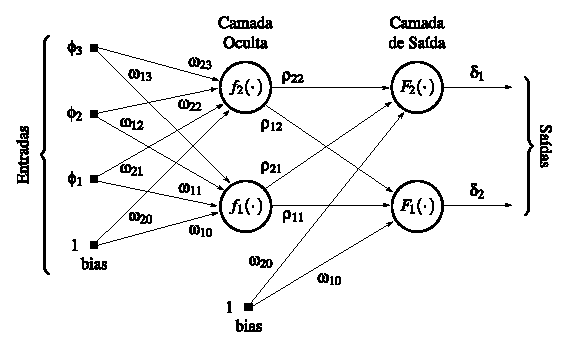
\includegraphics[width=0.7\textwidth]{imgs/rnas/eps/pmc}
\end{figure}

    Treinamento: Levenberg-Marquardt (LMA) -- Matlab\reg

\begin{itemize}
    \item Método Quase-Newton
    \item Rápida convergência
\end{itemize}

\end{frame}

\begin{frame}
    \frametitle{Arquitetura e modelo neural}

    Modelo neural: NNARX
\begin{figure}[htb]
\centering
    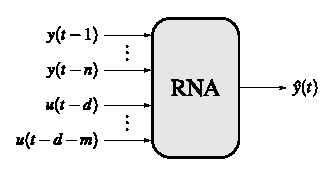
\includegraphics[width=0.5\textwidth]{imgs/rnas/eps/nnarx}
\end{figure}

    Ordem \implica número de regressores \implica complexidade

    \vspace{0.25cm}

    Avaliação das melhores redes \implica EMQ
\end{frame}

% Detecção e diagnóstico de falhas ---------------------------------------------
\section{Detecção e diagnóstico de falhas}
% ------------------------------------------------------------------------------
\subsection{Conceitos e terminologias}
\begin{frame}
    \frametitle{Conceitos e terminologias}

    Necessidades de otimização dos processos (qualidade, tempo de produção,
    custo, \ldots) \implica Importância dos sistemas de {\bf Detecção e 
    Diagnóstico de Falhas} (DDFs)

    \vspace{0.25cm}
    
    Sistemas de DDF:

\begin{itemize}
    \item Falha
    \item Erro
    \item Avaria
    \item Dependabilidade
    \item \ldots
\end{itemize}

    Existem muitas divergências relacionadas a definição desses termos
\end{frame}

% ------------------------------------------------------------------------------
\subsection{Dependabilidade}
\begin{frame}
    \frametitle{Dependabilidade}

    Sistemas computacionais podem ser caracterizados:

\begin{itemize}
    \item Funcionalidade
    \item Usabilidade
    \item Desempenho
    \item Custo
    \item \alert{Dependabilidade} (tradução literal de {\it dependability})
\end{itemize}

    \defin{{\bf Dependabilidade}: Capacidade de um sistema prestar um serviço
           que possa ser, justificadamente, confiável.}
\end{frame}

\begin{frame}
    \frametitle{Dependabilidade}

    Propriedades fundamentais da dependabilidade:

\begin{itemize}
    \small
    \item {\bf Disponibilidade:} Prontidão para uso;
    \item {\bf Confiabilidade:} Continuidade do serviço;
    \item \textbf{Proteção (\textit{safety}):} Não ocorrência de consequências
          catastróficas para o meio;
    \item {\bf Confidencialidade:} Não ocorrência da divulgação não-autorizada
          da informação;
    \item {\bf Integridade:} Não ocorrência de alterações indevidas da
          informação;
    \item {\bf Manutenção:} Aptidão para reparos e evolução.
\end{itemize}

    Associação da {\it integridade} com a {\it disponibilidade} \implica \textbf
    {Segurança (\textit{security})}

    \vspace{0.25cm}

    Utilização do termo dependabilidade de maneira mais conveniente \implica
    {\it Dependable System} \implica ``Sistema Confiável''
\end{frame}

\begin{frame}
    \frametitle{Dependabilidade}

    Sistemática de um sistema computacional confiável:

\begin{figure}[htb]
\centering
\footnotesize
\[
\text{Dependabilidade}
\left\{
\begin{array}{l}
\text{Atributos}
    \left\{
    \begin{array}{l}
        \text{Disponibilidade}\\
        \text{Confiabilidade}\\
        \text{Proteção}\\
        \text{Confidencialidade}\\
        \text{Integridade}\\
        \text{Manutenção}\\
        \text{Segurança}
    \end{array}
    \right.
\\
\\
\text{Ameaças}
    \left\{
    \begin{array}{l}
        \text{\color{red} Avaria ({\it failure})}\\
        \text{\color{red} Erro ({\it error})}\\
        \text{\color{red} Falha ({\it fault})}
    \end{array}
    \right.
\\
\\
\text{Meios}
    \left\{
    \begin{array}{l}
        \text{Prevenção}\\
        \text{Tolerância}\\
        \text{Supressão}\\
        \text{Previsão}
    \end{array}
    \right.
\end{array}
\right.
\]
\end{figure}

\end{frame}

% ------------------------------------------------------------------------------
\subsection{Falhas, erros e avarias}
\begin{frame}
    \frametitle{Falhas, erros e avarias}

    Falhas, erros e avarias são conceitos que não devem ser confundidos

\begin{itemize}
    \item \textbf{Avaria (\textit{failure}):} utilizado para indicar que houve
    um desvio do comportamento do sistema, o que o torna incapaz de fornecer o
    serviço para o qual foi designado
   
    \item \textbf{Erro (\textit{error}):} é relacionado com o estado do sistema
    e {\bf pode} levar a uma avaria (sequência de passos)
    
    \item \textbf{Falha (\textit{fault}):} é dita a causa dos erros, ou seja,
    está associada à noção de defeitos
\end{itemize}
\end{frame}

\begin{frame}
    \frametitle{Falhas, erros e avarias}

    Autores traduzem os termos {\it failure}, {\it error} e {\it fault} de
    maneira diferente

    \vspace{0.25cm}

    Exemplo:
\begin{itemize}
    \item {\it Failure} \implica Falha
    \item {\it Fault} \implica Falta
    \item Cuidado ao se referir aos sistemas de controle tolerante a {\bf
    falhas} 
    \begin{itemize}
        \item Lembrar que avarias ({\it failures}) não podem ser toleradas 
        \item Avaria = comprometimento funcional
    \end{itemize}
\end{itemize}
\end{frame}

\begin{frame}
    \frametitle{Falhas, erros e avarias}

    Mapa de conceitos:

\begin{figure}[htb]
\centering
    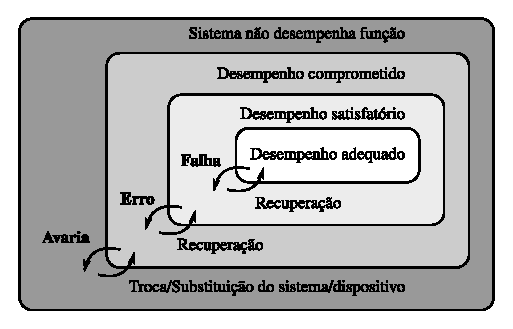
\includegraphics[width=0.55\textwidth]{imgs/detec_diag/eps/mapa_conceitos}
\[
\ldots
\quad\Longrightarrow\quad
\text{Falha} 
\quad\longrightarrow\quad
\text{Erro}
\quad\longrightarrow\quad
\text{Avaria}
\quad\Longrightarrow\quad
\text{Falha}
\quad\longrightarrow\quad
\ldots
\]
\end{figure}

\end{frame}

% ------------------------------------------------------------------------------
\subsection{Classificações de falhas}
\begin{frame}
    \frametitle{Classificações de falhas}

    Falhas podem ser classificadas sobre diversos aspectos

    \vspace{0.25cm}

    Classificação quanto ao tempo:

\begin{itemize}
    \item Abrupta
    \item Incipiente
    \item Intermitente
\end{itemize}

\begin{figure}[htb]
\centering
    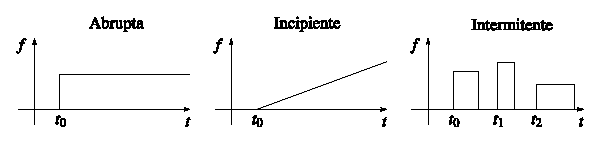
\includegraphics[width=0.8\textwidth]{imgs/detec_diag/eps/tipos_falha}
\end{figure}
\end{frame}

\begin{frame}
    \frametitle{Classificação de falhas}

    Podem agir em diversas partes do sistema

    \vspace{0.25cm}

    Maneira generalizada de se separar as áreas susceptíveis em um processo

    \vspace{0.25cm}

    Exemplos de falhas:

\begin{table}[htb]
\scriptsize
\centering
\begin{tabular}{|c|c|c|}
\hline
{\bf Sensores} & {\bf Atuadores} & {\bf Estrutura}\\
\hline
\hline
Erro de leitura & Erro de escrita & Erro de transmissão\\
\hline
Descalibramento & Erro de leitura & Perda de comunicação\\
\hline
Sensibilidade à ruído & Sensibilidade à ruído & Sensibilidade a ruído
(transmissor)\\
\hline
Queima & Queima & Queima (transmissor)\\
\hline
- & Atraso de transporte & Atraso de propagação de sinais\\
\hline
\end{tabular}
\end{table}

\end{frame}

% ------------------------------------------------------------------------------
\subsection{Detecção e diagnóstico}
\begin{frame}
    \frametitle{Detecção e diagnóstico}

    Objetivos de um sistema de DDF:

\begin{itemize}
    \item Detectar falhas
    \item Sugerir medidas corretivas ao operador \implica Garantir continuidade
          da operação do processo
\end{itemize}

    Na realidade, DDF consiste em 4 etapas:

\begin{figure}[htb]
\centering
    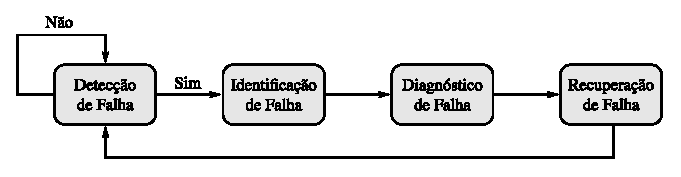
\includegraphics[width=0.8\textwidth]
    {imgs/detec_diag/eps/fases_monitoramento}
\end{figure}
\end{frame}

\begin{frame}
    \frametitle{Detecção e diagnóstico}

    O sistema proposto abrange as 3 primeiras etapas:

\begin{itemize}
    \item {\bf Detectar:} determinar se ocorreu ou não uma falha
    \item {\bf Identificar:} selecionar variáveis importantes para o diagnóstico
    \item {\bf Diagnosticar:} definir que falha ocorreu e fornecer o maior
          número de detalhes possíveis
    \begin{itemize}
        \item Intensidade
        \item Localização
        \item Momento de detecção
    \end{itemize}
\end{itemize}
\end{frame}

\begin{frame}
    \frametitle{Detecção e diagnóstico}

    Existem diversas técnicas para detecção e diagnóstico

    \vspace{0.25cm}

    Exemplos de técnicas/métodos de detecção:
\begin{itemize}
    \item Verificação de limites
    \item Modelos de sinais
    \item Equações de paridade
    \item Métodos de identificação
    \item Observadores/Estimadores de estado
\end{itemize}
\end{frame}

\begin{frame}
    \frametitle{Detecção e diagnóstico}

    Exemplos de técnicas/métodos de diagnóstico:
\begin{itemize}
    \item Classificação estatística
    \item Reconhecimento de padrões
    \item Métodos de aproximação
    \item Lógica de predicados
\end{itemize}

    Dentre as várias técnicas \implica RNAs (detecção e diagnóstico)
\end{frame}


% Sistema proposto -------------------------------------------------------------
\section{Sistema proposto}
% ------------------------------------------------------------------------------
\subsection{Estudo de caso}
\begin{frame}
    \frametitle{Estudo de caso}

    Sistemas de tanques acoplados da Quanser\reg

\begin{figure}[htb]
\centering
    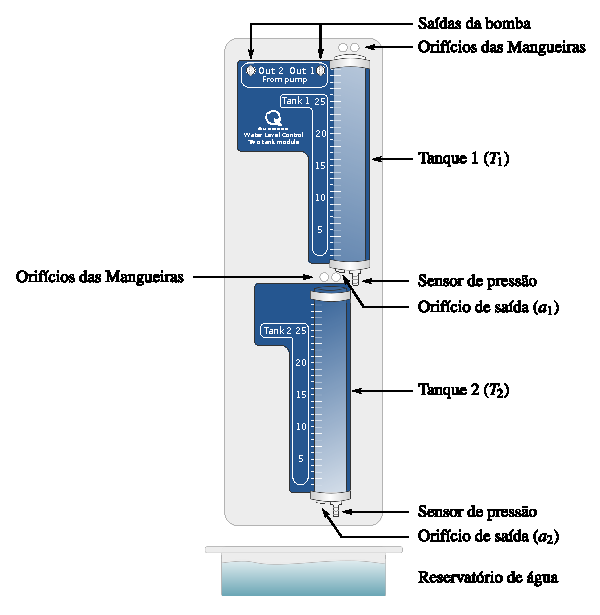
\includegraphics[width=0.6\textwidth]{imgs/sistema/eps/tanques}
\end{figure}
\end{frame}

\begin{frame}
    \frametitle{Estudo de caso}

    Sistema original:

\begin{itemize}
    \item Estrutura em acrílico
    \item Dois tanques
    \item Dois sensores de pressão
    \item Uma bomba de sucção bidirecional
    \item Mangueiras
    \item Orifícios (Entrada/Saída)
\end{itemize}

    Manual do fabricante \implica Sugere três configurações

\begin{itemize}
    \item Controlar $L_1$ (alimentação direta em $T_1$)
    \item Controlar $L_2$ (alimentação indireta em $T_1$)
    \item Controlar $L_2$ (alimentação em $T_1$ e $T_2$)
\end{itemize}

    Todas as três configurações \implica Sistema SISO
\end{frame}

\begin{frame}
    \frametitle{Estudo de caso}

    Modelo matemático (EDOs não-lineares):

\begin{eqnarray}
\dot{L_1} & = & \alert<2>{\frac{K_m}{A}V_p} -
                \alert<3>{\left[\frac{a_1}{A}\sqrt{2g}\right]\sqrt{L_1}}
\nonumber\\
\dot{L_2} & = & \alert<4>{\left[\frac{a_1}{A}\sqrt{2g}\right]\sqrt{L_1}} -
                \alert<5>{\left[\frac{a_2}{A}\sqrt{2g}\right]\sqrt{L_2}}
\nonumber
\end{eqnarray}

\uncover<6->
{
    Modificações do modelo:

\begin{itemize}
    \item Introdução de uma nova bomba
    \item Possibilidade de controlar $L_1$ e $L_2$ simultaneamente
    \item Sistema SISO \implica Sistema MIMO
\end{itemize}
}

\end{frame}

\begin{frame}
    \frametitle{Estudo de caso}

    Modelo matemático (EDOs não-lineares):

\begin{eqnarray}
\dot{L_1} & = & \frac{K_m}{A}\alert<1>{V_{p_{\tiny 1}}} -
                \left[\frac{a_1}{A}\sqrt{2g}\right]\sqrt{L_1}
\nonumber\\
\dot{L_2} & = & \left[\frac{a_1}{A}\sqrt{2g}\right]\sqrt{L_1} -
                \left[\frac{a_2}{A}\sqrt{2g}\right]\sqrt{L_2}
                \alert<1>{+ \frac{K_m}{A}V_{p_{\tiny 2}}}
\nonumber
\end{eqnarray}

    Modificações do modelo:

\begin{itemize}
    \item Introdução de uma nova bomba
    \item Possibilidade de controlar $L_1$ e $L_2$ simultaneamente
    \item Sistema SISO \implica Sistema MIMO
\end{itemize}
\end{frame}

\begin{frame}
    \frametitle{Estudo de caso}

    Novas configurações:
\begin{figure}[htb]
\centering
\subfigure
{
    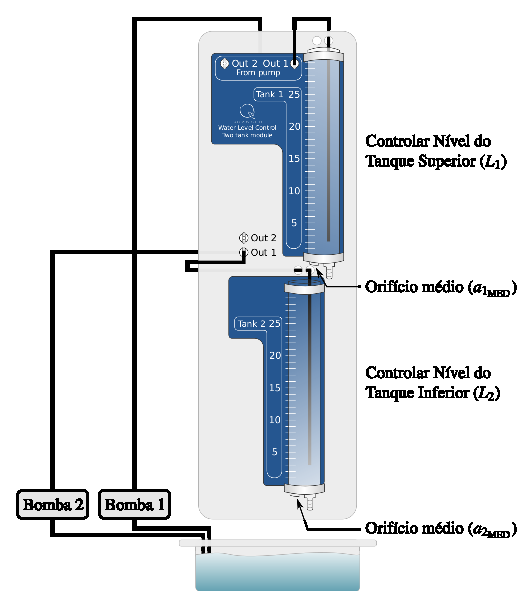
\includegraphics[width=0.47\textwidth]{imgs/sistema/eps/nova_config_1}
}
\quad
\subfigure
{
    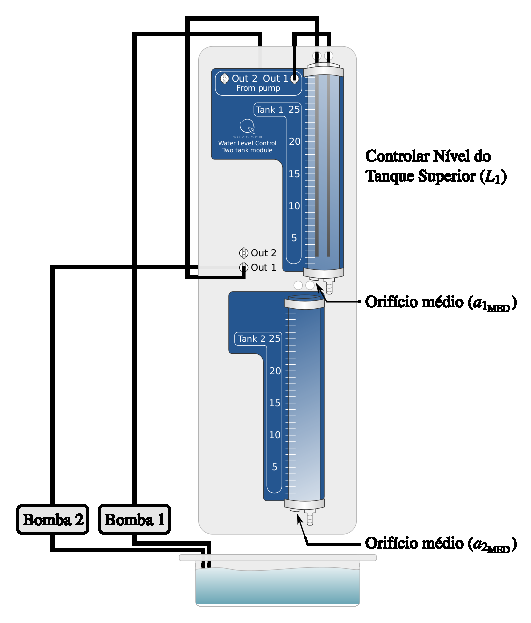
\includegraphics[width=0.47\textwidth]{imgs/sistema/eps/nova_config_2}
}
\end{figure}
\end{frame}

% ------------------------------------------------------------------------------
\subsection{Estrutura do sistema e limitações}
\begin{frame}
    \frametitle{Estrutura do sistema e limitações}

    Estrutura do sistema proposto:

\begin{figure}[htb]
\centering
    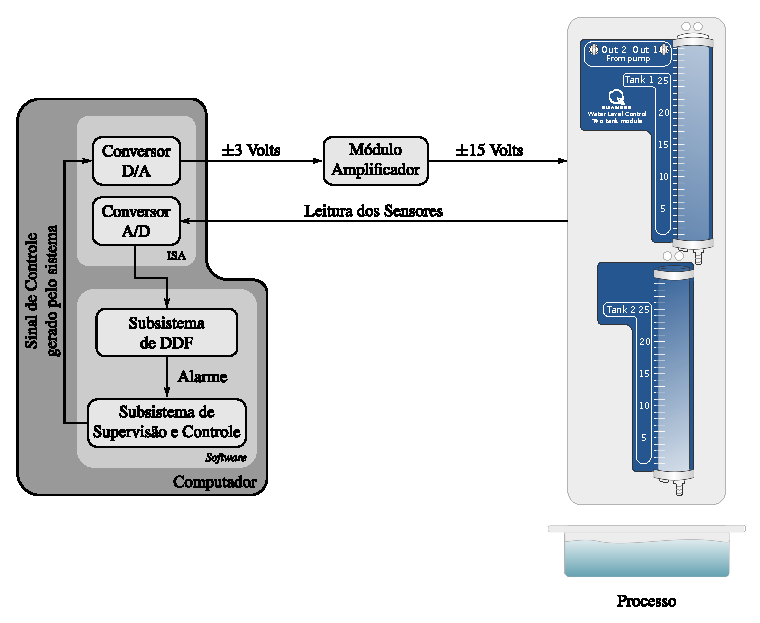
\includegraphics[width=0.8\textwidth]{imgs/sistema/eps/func_sistema}
\end{figure}
\end{frame}

\begin{frame}
    \frametitle{Estrutura do sistema e limitações}

    Estrutura do sistema proposto:

\begin{figure}[htb]
\centering
    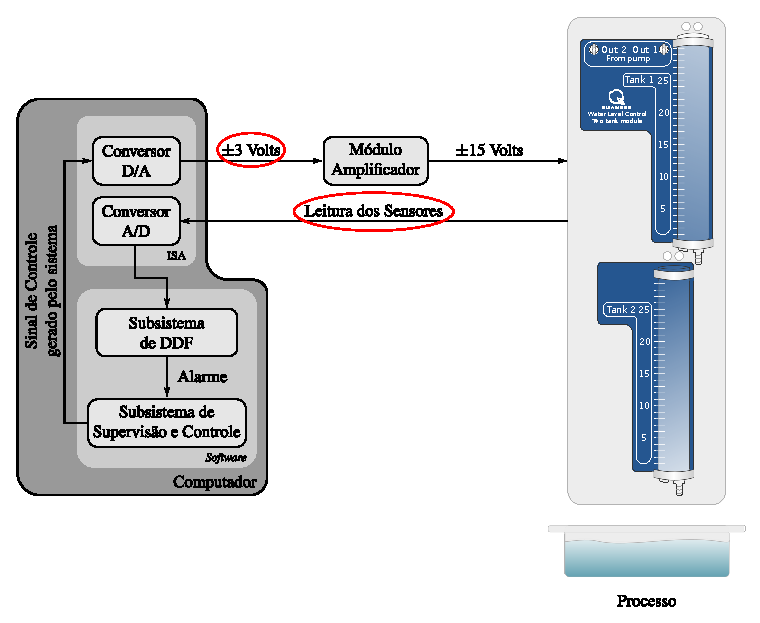
\includegraphics[width=0.8\textwidth]{imgs/sistema/eps/func_sistema_mod}
\end{figure}
\end{frame}

% ------------------------------------------------------------------------------
\subsection{Simulações}
\begin{frame}
    \frametitle{Simulações}

    EDOs do modelo simuladas com Runge-Kutta 4\textordfeminine\ ordem

    \vspace{0.25cm}

    Falhas simuladas através de modificações na simulação

\begin{itemize}
    \item Ex.: Ruído no sensor \implica Valor lido no sensor $\pm$ Ruído 
\end{itemize}

    Grupos de falhas selecionadas:

\begin{table}[!htb]
\small
\centering
\begin{tabular}{|c|c|c|}
\hline
{\bf Grupo} & {\bf Tipo de falha} & {\bf Sigla}\\
\hline
\hline
0 & Não há falhas & SF\\
\hline
1 & Falha do sensor & FSe\\
\hline
2 & Falha do atuador & FA\\
\hline
\multirow{2}{*}{3} & 
Falha estrutural ou & 
\multirow{2}{*}{FSi}\\
&
Falha do sistema & 
\\
\hline
\end{tabular}
\end{table}
\end{frame}

\begin{frame}
    \frametitle{Simulações}

    Classificação das falhas:

\begin{table}[!htb]
\scriptsize
\centering
\begin{tabular}{|c|c|c|c|c|}
\hline
{\bf Grupo} & {\bf Classe} & {\bf Denominação} & {\bf Variante} & {\bf Sigla}\\
\hline
\hline
1 & 1 & Descalibramento & Ganho & FSeDG\\
\hline
1 & 1 & Descalibramento & Nível DC ({\it offset}) & FSeDO\\
\hline
1 & 2 & Sensibilidade & Ruído & FSeSR\\
\hline
1 & 3 & Queima & -- & FSeQ\\
\hline
\hline
2 & 1 & Descalibramento & Ganho & FADG\\
\hline
2 & 1 & Descalibramento & Nível DC ({\it offset}) & FADO\\
\hline
2 & 2 & Sensibilidade & Ruído & FASR\\
\hline
2 & 3 & Variação & Constante da bomba ($K_m$) & FAVK\\
\hline
2 & 4 & Queima & -- & FAQ\\
\hline
\hline
3 & 3 & Vazamento & Tanque & FSiVzT\\
\hline
3 & 2 & Variação & Orifício de saída & FSiVrOS\\
\hline
3 & 2 & Variação & Ganho do módulo de potência & FSiVrGMP\\
\hline
3 & 1 & Entupimento & Orifício de saída & FSiEOS\\
\hline
\end{tabular}
\end{table}
\end{frame}

\begin{frame}
    \frametitle{Simulações}

    Sistema desenvolvido para as simulações (Qt/C++)

\begin{itemize}
    \item Configuração através de arquivo
    \item Simulação em tempo real ou Simulação rápida
    \item Comunicação com a planta real (Sockets TCP/IP)
    \item Exportação de dados
    \item Exportação de imagens
\end{itemize}

\end{frame}

% ------------------------------------------------------------------------------
\subsection{Estruturas neurais}
\begin{frame}
    \frametitle{Estruturas neurais -- Identificação}

    Duas propostas de identificação do modelo:

\begin{itemize}
    \item Identificação global (uma RNA para $T_1$ e $T_2$)
    \item Identificação individual (uma RNA para cada tanque)
\end{itemize}

\begin{figure}[htb]
\centering
    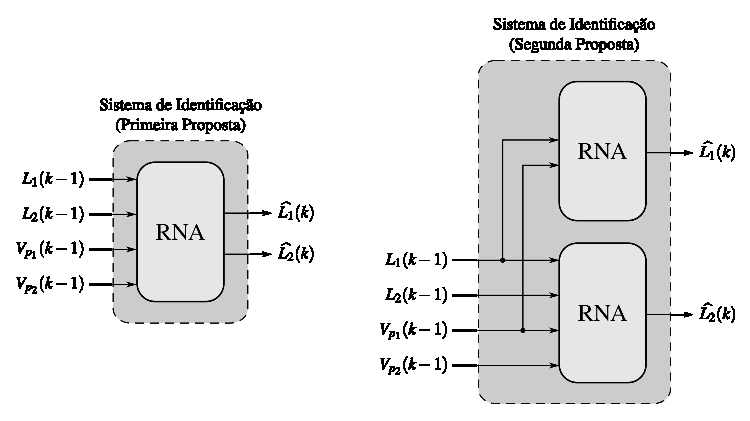
\includegraphics[width=0.8\textwidth]{imgs/sistema/eps/sist_ident}
\end{figure}

\end{frame}

\begin{frame}
    \frametitle{Estruturas neurais -- Detecção}

    Para detecção mais eficiente \implica Utilização de resíduos:

\begin{figure}[htb]
\centering
    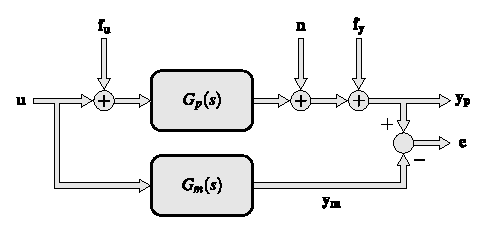
\includegraphics[width=0.65\textwidth]{imgs/detec_diag/eps/residuos}
\end{figure}

    Duas propostas de detecção:

\begin{itemize}
    \item RNA única (todas as falhas)
    \item Conjunto de especialistas (uma RNA para cada falha)
\end{itemize}
    
\end{frame}

\begin{frame}
    \frametitle{Estruturas neurais -- Detecção}

    Primeira proposta:
\begin{figure}[htb]
\centering
    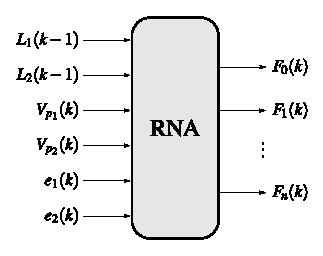
\includegraphics[width=0.35\textwidth]{imgs/sistema/eps/detec_prop_1}
\end{figure}

    Saída \implica Palavra binária de $n$ bits
    
\end{frame}

\begin{frame}
    \frametitle{Estruturas neurais -- Detecção}

    Segunda proposta:

\begin{columns}
\column{0.57\textwidth}
\begin{figure}[htb]
\centering
    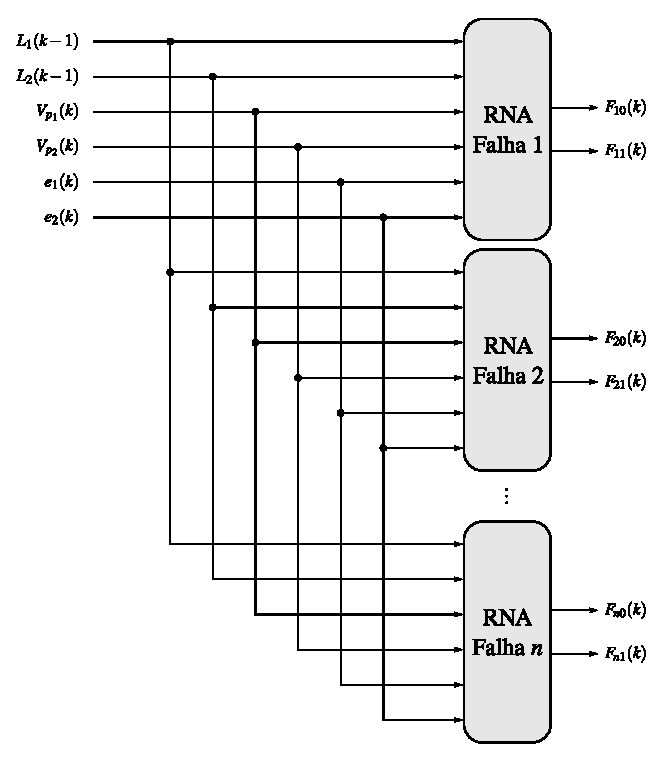
\includegraphics[width=0.95\textwidth]{imgs/sistema/eps/detec_prop_2}
\end{figure}

\column{0.45\textwidth}
    Saída \implica 2 bits 
\begin{itemize}
    \item Sem falha
    \item Falha $T_1$
    \item Falha $T_2$
    \item Falha $T_1$ + $T_2$
\end{itemize}
\end{columns}
\end{frame}

\begin{frame}
    \frametitle{Estruturas neurais -- Detecção}

    Vantagens em se utilizar a segunda proposta:

\begin{itemize}
    \item Possibilidade de utilizar entradas diferentes para cada falha
    \item Modificar a estrutura das entradas
    \begin{itemize}
        \item Proposta 1: retreinamento completo
        \item Proposta 2: retreinamento somente de uma das falha
    \end{itemize}
    \item Pós-processamento da informação
    \begin{itemize}
        \item Proposta 1: 
        \begin{itemize}
            \item N\textordmasculine\ falhas \implica N\textordmasculine\
                  palavras \implica N\textordmasculine\ combinações \implica 
                  N\textordmasculine\ bits
        \end{itemize}
        \item Proposta 2: 
        \begin{itemize}
            \item praticamente não há decodificação da palavra (2 bits)
        \end{itemize}
    \end{itemize}
    \item Facilidadade de acoplamento dos sinais de saída na segunda proposta
\end{itemize}

\end{frame}

% ------------------------------------------------------------------------------
\subsection{Composição do sistema}
\begin{frame}
    \frametitle{Composição do sistema}

\begin{figure}[htb]
\centering
    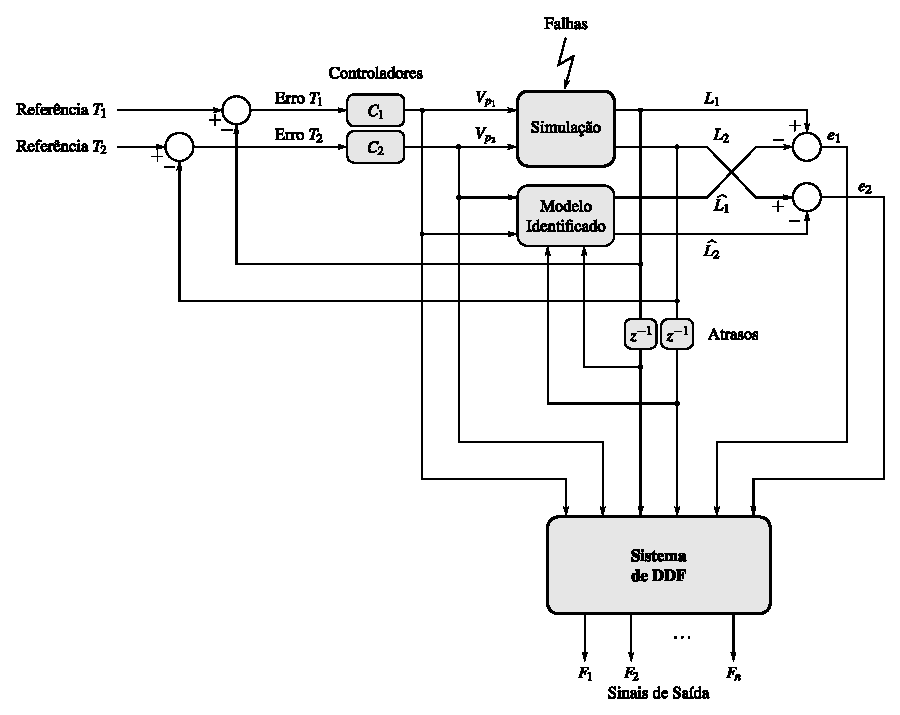
\includegraphics[width=0.9\textwidth]{imgs/sistema/eps/composicao_mod_0}
\end{figure}
\end{frame}

\begin{frame}
    \frametitle{Composição do sistema}

\begin{figure}[htb]
\centering
    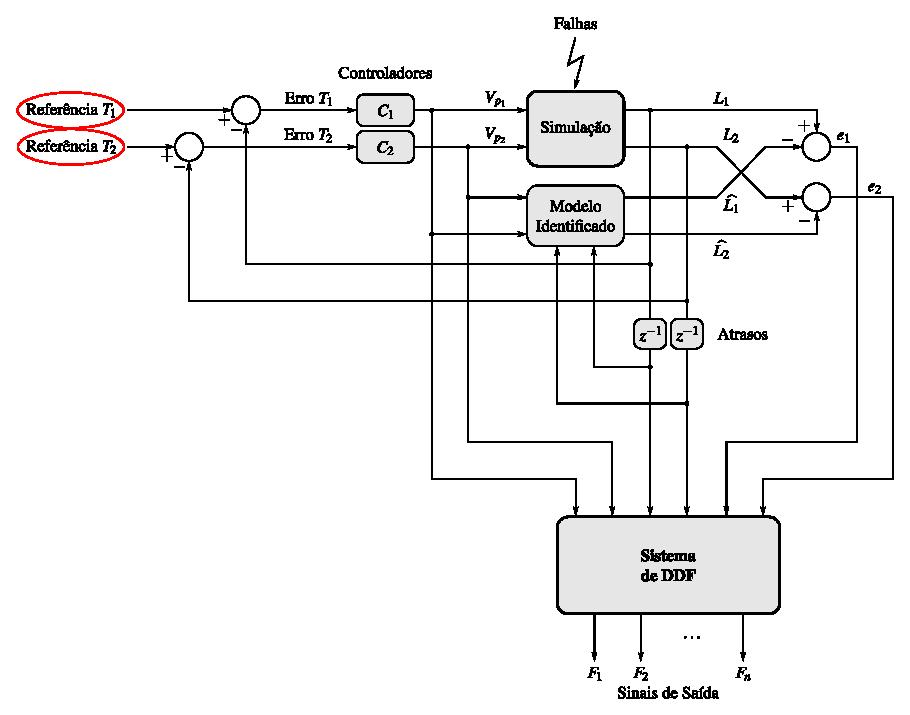
\includegraphics[width=0.9\textwidth]{imgs/sistema/eps/composicao_mod_1}
\end{figure}
\end{frame}

\begin{frame}
    \frametitle{Composição do sistema}

\begin{figure}[htb]
\centering
    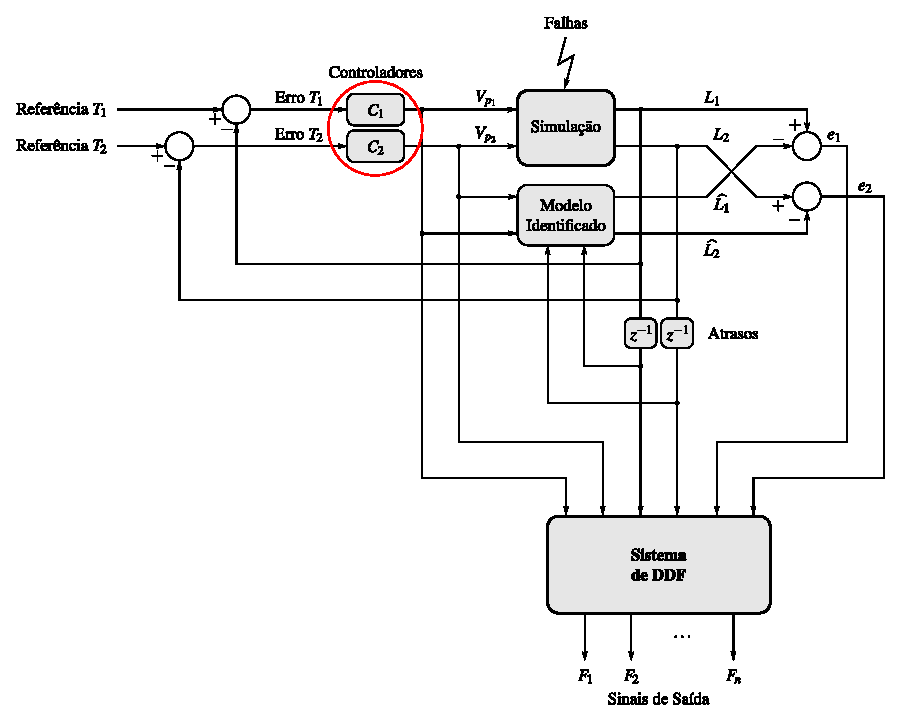
\includegraphics[width=0.9\textwidth]{imgs/sistema/eps/composicao_mod_2}
\end{figure}
\end{frame}

\begin{frame}
    \frametitle{Composição do sistema}

\begin{figure}[htb]
\centering
    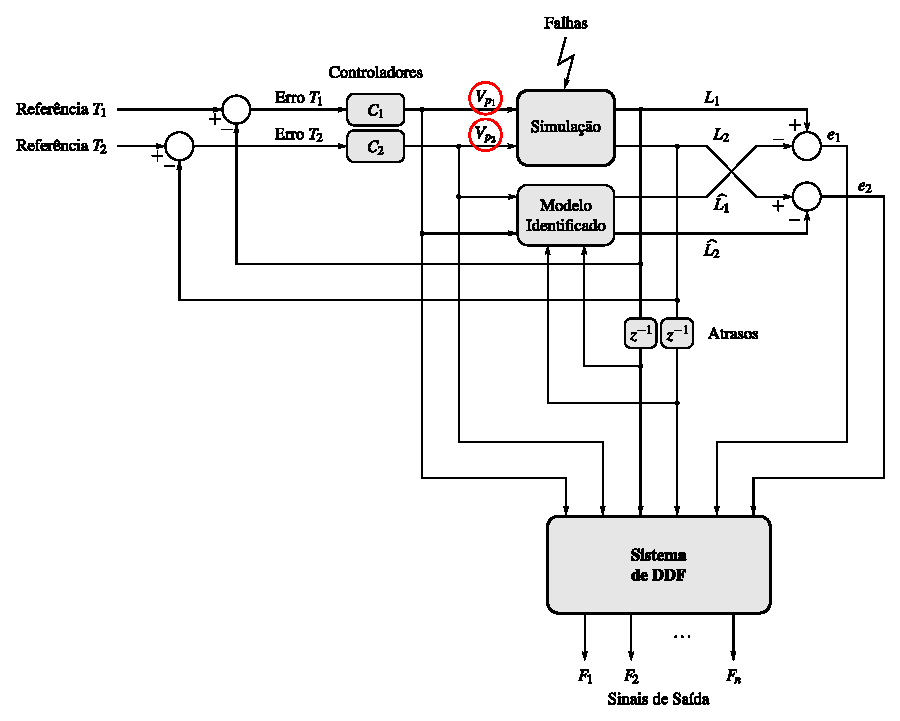
\includegraphics[width=0.9\textwidth]{imgs/sistema/eps/composicao_mod_3}
\end{figure}
\end{frame}

\begin{frame}
    \frametitle{Composição do sistema}

\begin{figure}[htb]
\centering
    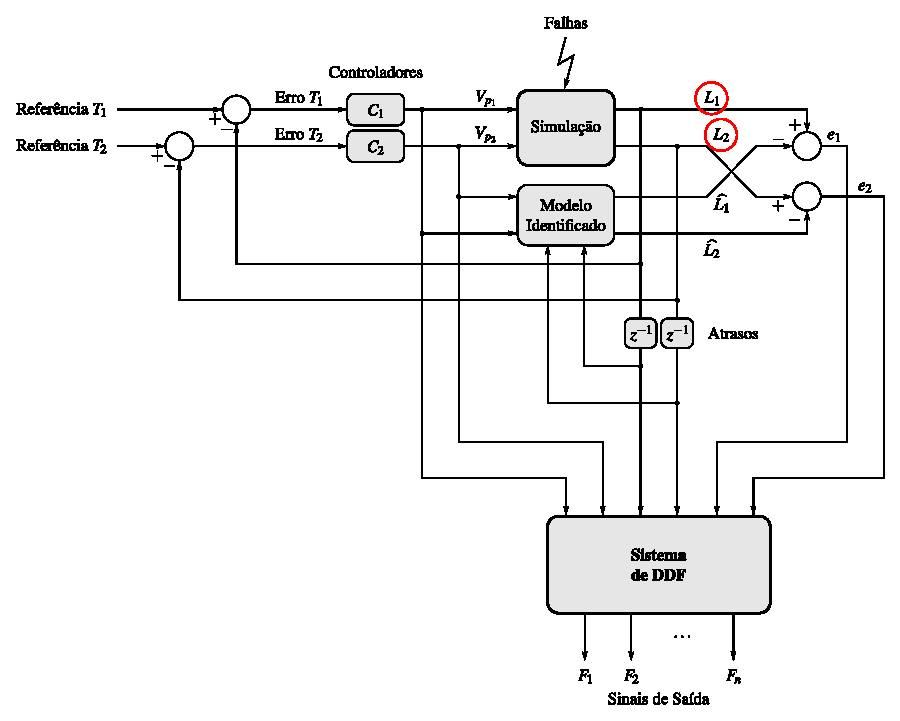
\includegraphics[width=0.9\textwidth]{imgs/sistema/eps/composicao_mod_4}
\end{figure}
\end{frame}

\begin{frame}
    \frametitle{Composição do sistema}

\begin{figure}[htb]
\centering
    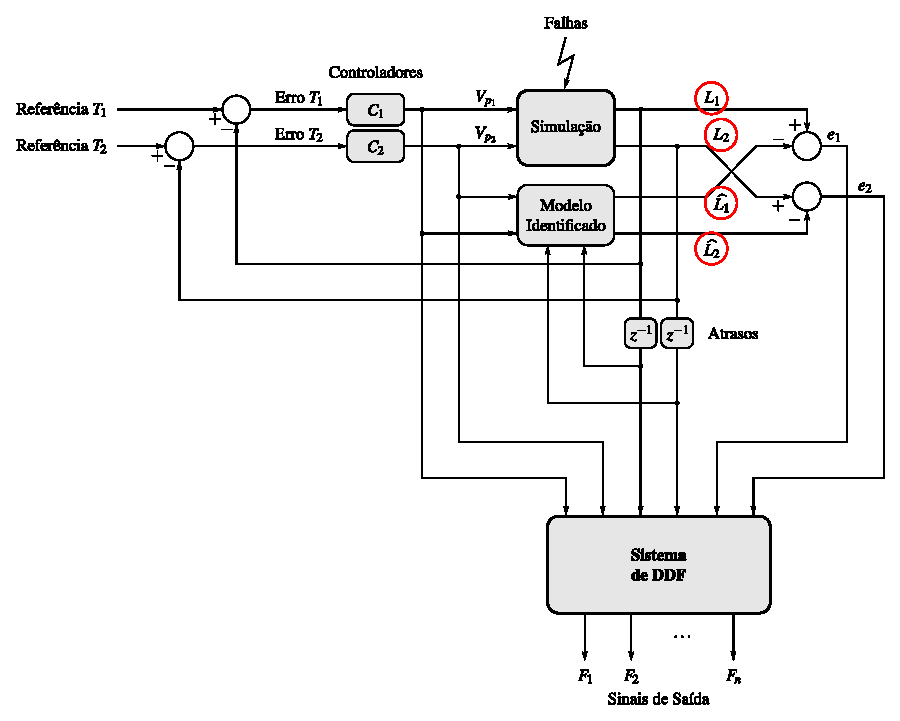
\includegraphics[width=0.9\textwidth]{imgs/sistema/eps/composicao_mod_5}
\end{figure}
\end{frame}

\begin{frame}
    \frametitle{Composição do sistema}

\begin{figure}[htb]
\centering
    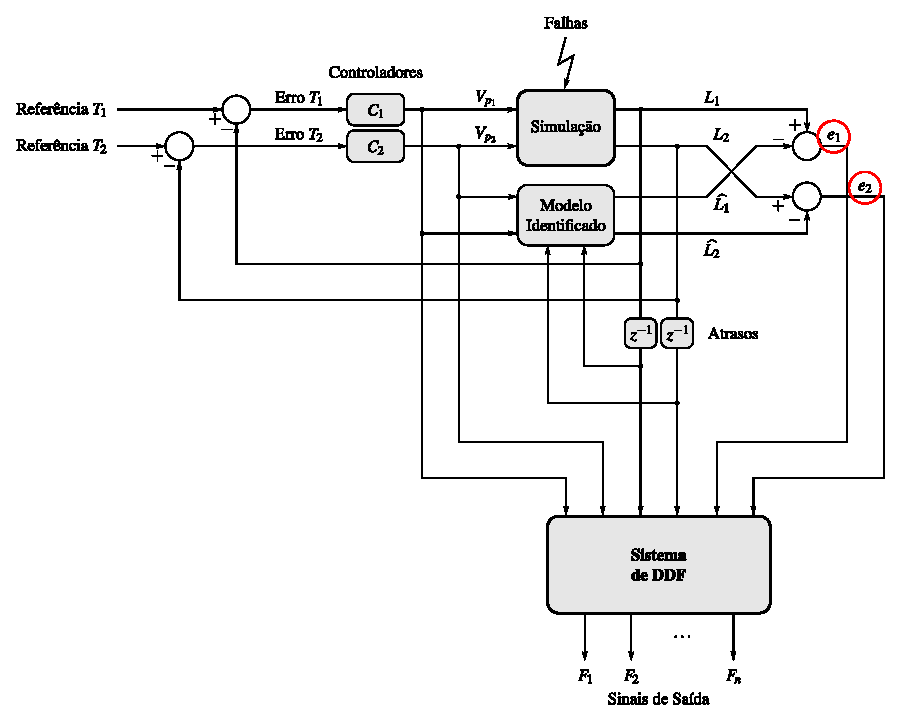
\includegraphics[width=0.9\textwidth]{imgs/sistema/eps/composicao_mod_6}
\end{figure}
\end{frame}

\begin{frame}
    \frametitle{Composição do sistema}

\begin{figure}[htb]
\centering
    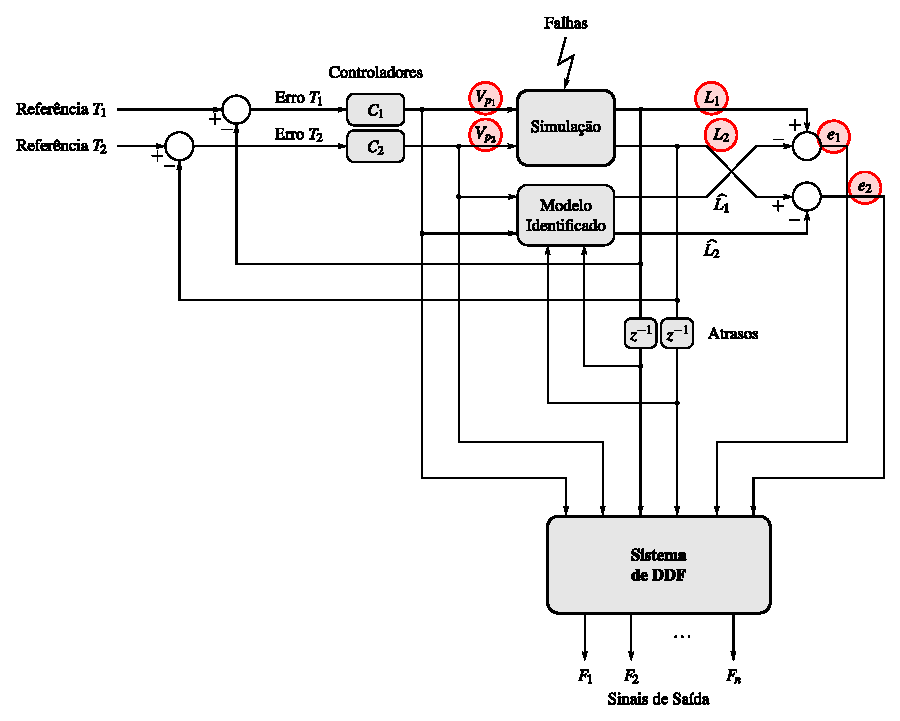
\includegraphics[width=0.9\textwidth]{imgs/sistema/eps/composicao_mod_7}
\end{figure}
\end{frame}

\begin{frame}
    \frametitle{Composição do sistema}

\begin{figure}[htb]
\centering
    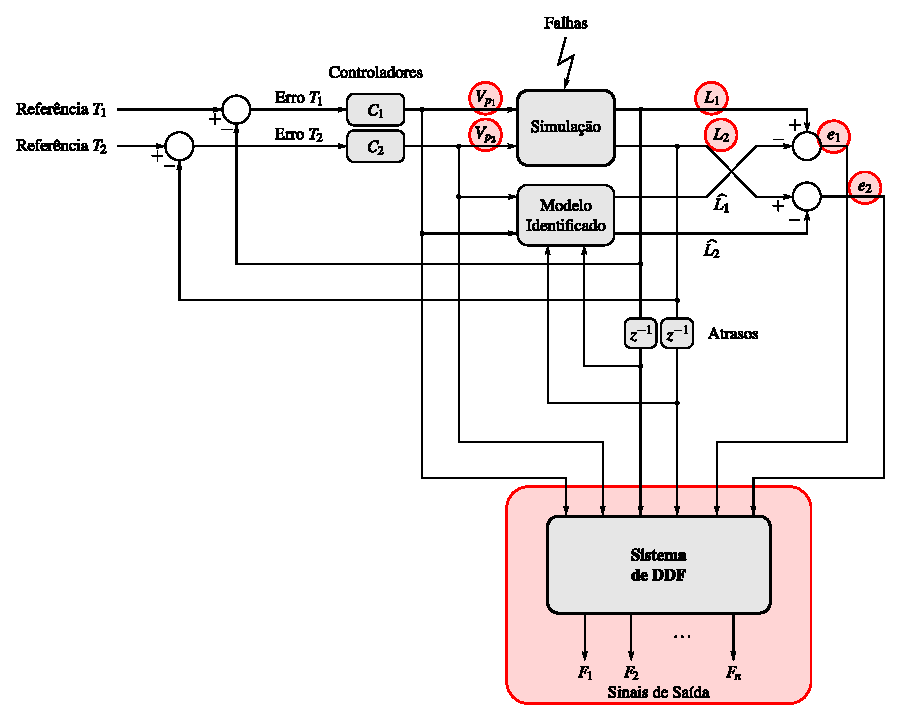
\includegraphics[width=0.9\textwidth]{imgs/sistema/eps/composicao_mod_8}
\end{figure}
\end{frame}

% Resultados parciais ----------------------------------------------------------
\section{Resultados parciais}
% ------------------------------------------------------------------------------
\subsection{Coleta dos dados}

\begin{frame}
    \frametitle{Coleta dos dados}

    Após ter selecionado as falhas e as estruturas neurais:

\begin{itemize}
    \item Excitação da planta com sinais PRBS dentro de um {\it range}
          especificado
    \begin{itemize}
        \item Referências: 0 a 30 cm
        \item Ruído: $\pm 2\%$
        \item $K_m' = \pm 20\% K_m$
        \item ...
    \end{itemize}
    \item Simulação do sistema sem falhas \implica identificação do modelo
    \item Simulação com falhas (individual -- proposta 2)
\end{itemize}
\end{frame}

% ------------------------------------------------------------------------------
\subsection{Treinamento e validação das RNAs}
\begin{frame}
    \frametitle{Treinamento e validação das RNAs}

    Treinamento:

\begin{itemize}
    \item Identificação: 10 minutos (6000 amostras)
    \item Detecção: 20 minutos (12000 amostras)
\end{itemize}

    Número de redes treinadas:

\begin{table}[htb]
\scriptsize
\centering
\begin{tabular}{|c|c|c|c|c|}
\hline
% Linha 1
\multirow{2}{*}{\bf Proposta} & 
\multirow{2}{*}{\bf Ordem} & 
{\bf Neurônios na} & 
{\bf Número de} & 
\multirow{2}{*}{\bf Total}\\
% Linha 2
& & {\bf camada oculta} & {\bf redes treinadas} &\\
\hline
\hline
\multicolumn{5}{|l|}{{\bf Identificação}}\\
\hline
\multirow{3}{*}{1} & 2 & 6/8/10 & \multirow{3}{*}{6} & \multirow{3}{*}{54}\\
\cline{2-3}
& 3 & 8/12/16 & &\\
\cline{2-3}
& 4 & 10/16/22 & &\\
\hline
\multirow{3}{*}{2} & 2 & 2/4/6 -- 6/8/10 & 
\multirow{3}{*}{6} & \multirow{3}{*}{108}\\
\cline{2-3}
& 3 & 4/6/8 -- 8/12/16 & & \\
\cline{2-3}
& 4 & 6/8/10 -- 10/16/22 & & \\
\hline
\multicolumn{5}{|l|}{{\bf Detecção}}\\
\hline
\multirow{3}{*}{2} & 2 & 8/12/16 & 
\multirow{3}{*}{6/falha} &
\multirow{3}{*}{702}\\
\cline{2-3}
& 3 & 14/18/22 & &\\
\cline{2-3}
& 4 & 20/24/28 & &\\
\hline
\hline
\multicolumn{4}{|r|}{{\bf Total}} & 864\\
\hline
\end{tabular}
\end{table}

\end{frame}

% ------------------------------------------------------------------------------
\subsection{Melhores redes}
\begin{frame}
    \frametitle{Melhores redes}

    RNAs de Identificação:

\begin{itemize}
    \item 3 validações
    \item Média dos EMQs em $L_1$ e $L_2$
    \item Critério de seleção EMQ = EMQ $L_1$ + EMQ $L_2$
\end{itemize}

\begin{table}[htb]
\footnotesize
\centering
\begin{threeparttable}
\begin{tabular}{|c|c|c|c|c|c|c|}
\hline
% Linha 1
{\bf Proposta} & 
{\bf Ordem} & 
{\bf NCO\tnote{$*$}} & 
{\bf Treinamento} &
{\bf EMQ $\mathbf{L_1}$} & 
{\bf EMQ $\mathbf{L_2}$} & 
{\bf EMQ}\\
\hline
\hhline\\
\multirow{3}{*}{1} &
\cellcolor[gray]{0.85}2 &
\cellcolor[gray]{0.85}8 &
\cellcolor[gray]{0.85}2 &
\cellcolor[gray]{0.85}4,39e-7 &
\cellcolor[gray]{0.85}3,29e-6 &
\cellcolor[gray]{0.85}3,73e-6\\
\hhline{~------}
&3 & 12 & 5 & 1,38e-5 & 1,46e-5 & 2,84e-5\\
\cline{2-7}
&4 & 22 & 4 & 1,40e-6 & 2,60e-6 & 4,01e-6\\
\hline
\multirow{3}{*}{2} & 2 & 2 -- 6 & 2 & 5,06e-6 & 7,26e-6 & 1,23e-5\\
\cline{2-7}
& 3 & 6 -- 12 & 1 & 5,48e-6 & 1,81e-7 & 5,66e-6\\
\cline{2-7}
& 4 & 10 -- 22 & 3 & 5,12e-6 & 9,46e-6 & 1,45e-5\\
\hline
\end{tabular}
\begin{tablenotes}
\item [$*$] Número de neurônios na camada oculta.
\end{tablenotes}
\end{threeparttable}
\end{table}
\end{frame}

\begin{frame}
    \frametitle{Melhores redes}

RNAs de detecção:

\begin{itemize}
    \item Selecionadas de modo semelhante: 3 validações
    \item Critérios de seleção
    \begin{itemize}
        \item Número de erros de tipo I e tipo II (falsos positivos/negativos)
        \item Porcentagem total de erros sobre as 3 validações
    \end{itemize}
\end{itemize}

Simulação final:    

\begin{itemize}
    \item Utilização das melhores redes de identificação e detecção
    \item Cada falha \implica 1 minuto e 45 segundos
\begin{figure}[htb]
\centering
    
\includegraphics[width=0.8\textwidth]{imgs/resultados/eps/intervalos}
\end{figure}
    \item Valores das falhas \implica mantidos fixos dentro do {\it
          range} estabelecido para o treinamento
\end{itemize}
\end{frame}

% ------------------------------------------------------------------------------
\subsection{Resultados das simulações}
\begin{frame}
    \frametitle{Resultados das simulações}

\begin{table}[htb]
\scriptsize
\begin{tabular}{|c|c|c|c|c|c|c|c|}
\hline
\multirow{2}{*}{\bf Falha} &
\multirow{2}{*}{\bf Ordem} &
\multirow{2}{*}{\bf NCO} &
\multirow{2}{*}{\bf Trein.} &
\multirow{2}{*}{\bf Acertos} &
{\bf Erros de} & {\bf Erros de} & {\bf Total de}\\
& & & & & {\bf tipo I} & {\bf tipo II} & {\bf erros}\\
\hline
\hline
FSeDG & 4 & 28 & 2 & 23491,33 & 203,33 & 305,33 & 2,12\%\\
\hline
FSeDO & 4 & 28 & 5 & 23890,33 & 8,66 & 101 & 0,46\%\\
\hline
FSeSR & 4 & 20 & 3 & 23317 & 324,66 & 358,33 & 2,84\%\\
\hline
FSeQ & 4 & 20 & 4 & 23994 & 0,66 & 5,33 & 0,02\%\\
\hline
FADG & 2 & 8 & 3 & 20710,33 & 1626,66 & 1663 & 13,7\%\\
\hline
FADO & 4 & 28 & 3 & 23075,33 & 635,66 & 289 & 3,85\%\\
\hline
\alert<2->{FASR} & 2 & 8 & 6 & 14153,33 & 3407 & 6439,66 & \alert<2->{41,03\%}\\
\hline
FAVK & 2 & 8 & 5 & 20764,66 & 1551,33 & 1684 & 13,48\%\\
\hline
FAQ & 4 & 28 & 6 & 23980 & 2,33 & 17,66 & 0,083\%\\
\hline
FSiVzT & 4 & 24 & 1 & 23774,33 & 74 & 151,66 & 0,94\%\\
\hline
FSiVrOS & 2 & 8 & 3 & 22465,33 & 437 & 1097,66 & 6,39\%\\
\hline
FSiVrGMP & 4 & 20 & 2 & 20905,66 & 1979,66 & 1114,66 & 12,89\%\\
\hline
\alert<2->{FSiEOS} & 2 & 12 & 4 & 23995,66 & 1 & 3,33 & \alert<2->{0,018\%}\\
\hline
\end{tabular}
\end{table}
\end{frame}

\begin{frame}
    \frametitle{Resultados das simulações}

\footnotesize Simulação da FSeDG com o ganho reduzido a 80\% do valor original:

\begin{figure}[htb]
\footnotesize
\centering
\scalebox{0.68}{% GNUPLOT: LaTeX picture with Postscript
\begingroup
  \makeatletter
  \providecommand\color[2][]{%
    \GenericError{(gnuplot) \space\space\space\@spaces}{%
      Package color not loaded in conjunction with
      terminal option `colourtext'%
    }{See the gnuplot documentation for explanation.%
    }{Either use 'blacktext' in gnuplot or load the package
      color.sty in LaTeX.}%
    \renewcommand\color[2][]{}%
  }%
  \providecommand\includegraphics[2][]{%
    \GenericError{(gnuplot) \space\space\space\@spaces}{%
      Package graphicx or graphics not loaded%
    }{See the gnuplot documentation for explanation.%
    }{The gnuplot epslatex terminal needs graphicx.sty or graphics.sty.}%
    \renewcommand\includegraphics[2][]{}%
  }%
  \providecommand\rotatebox[2]{#2}%
  \@ifundefined{ifGPcolor}{%
    \newif\ifGPcolor
    \GPcolortrue
  }{}%
  \@ifundefined{ifGPblacktext}{%
    \newif\ifGPblacktext
    \GPblacktexttrue
  }{}%
  % define a \g@addto@macro without @ in the name:
  \let\gplgaddtomacro\g@addto@macro
  % define empty templates for all commands taking text:
  \gdef\gplbacktext{}%
  \gdef\gplfronttext{}%
  \makeatother
  \ifGPblacktext
    % no textcolor at all
    \def\colorrgb#1{}%
    \def\colorgray#1{}%
  \else
    % gray or color?
    \ifGPcolor
      \def\colorrgb#1{\color[rgb]{#1}}%
      \def\colorgray#1{\color[gray]{#1}}%
      \expandafter\def\csname LTw\endcsname{\color{white}}%
      \expandafter\def\csname LTb\endcsname{\color{black}}%
      \expandafter\def\csname LTa\endcsname{\color{black}}%
      \expandafter\def\csname LT0\endcsname{\color[rgb]{1,0,0}}%
      \expandafter\def\csname LT1\endcsname{\color[rgb]{0,1,0}}%
      \expandafter\def\csname LT2\endcsname{\color[rgb]{0,0,1}}%
      \expandafter\def\csname LT3\endcsname{\color[rgb]{1,0,1}}%
      \expandafter\def\csname LT4\endcsname{\color[rgb]{0,1,1}}%
      \expandafter\def\csname LT5\endcsname{\color[rgb]{1,1,0}}%
      \expandafter\def\csname LT6\endcsname{\color[rgb]{0,0,0}}%
      \expandafter\def\csname LT7\endcsname{\color[rgb]{1,0.3,0}}%
      \expandafter\def\csname LT8\endcsname{\color[rgb]{0.5,0.5,0.5}}%
    \else
      % gray
      \def\colorrgb#1{\color{black}}%
      \def\colorgray#1{\color[gray]{#1}}%
      \expandafter\def\csname LTw\endcsname{\color{white}}%
      \expandafter\def\csname LTb\endcsname{\color{black}}%
      \expandafter\def\csname LTa\endcsname{\color{black}}%
      \expandafter\def\csname LT0\endcsname{\color{black}}%
      \expandafter\def\csname LT1\endcsname{\color{black}}%
      \expandafter\def\csname LT2\endcsname{\color{black}}%
      \expandafter\def\csname LT3\endcsname{\color{black}}%
      \expandafter\def\csname LT4\endcsname{\color{black}}%
      \expandafter\def\csname LT5\endcsname{\color{black}}%
      \expandafter\def\csname LT6\endcsname{\color{black}}%
      \expandafter\def\csname LT7\endcsname{\color{black}}%
      \expandafter\def\csname LT8\endcsname{\color{black}}%
    \fi
  \fi
  \setlength{\unitlength}{0.0500bp}%
  \begin{picture}(7200.00,5040.00)%
    \gplgaddtomacro\gplbacktext{%
      \csname LTb\endcsname%
      \put(726,3150){\makebox(0,0)[r]{\strut{} 5}}%
      \csname LTb\endcsname%
      \put(726,3780){\makebox(0,0)[r]{\strut{} 10}}%
      \csname LTb\endcsname%
      \put(726,4409){\makebox(0,0)[r]{\strut{} 15}}%
      \csname LTb\endcsname%
      \put(726,5039){\makebox(0,0)[r]{\strut{} 20}}%
      \csname LTb\endcsname%
      \put(921,2237){\makebox(0,0){\strut{}}}%
      \csname LTb\endcsname%
      \put(1771,2237){\makebox(0,0){\strut{}}}%
      \csname LTb\endcsname%
      \put(2620,2237){\makebox(0,0){\strut{}}}%
      \csname LTb\endcsname%
      \put(3470,2237){\makebox(0,0){\strut{}}}%
      \csname LTb\endcsname%
      \put(4320,2237){\makebox(0,0){\strut{}}}%
      \csname LTb\endcsname%
      \put(5170,2237){\makebox(0,0){\strut{}}}%
      \csname LTb\endcsname%
      \put(6019,2237){\makebox(0,0){\strut{}}}%
      \csname LTb\endcsname%
      \put(6869,2237){\makebox(0,0){\strut{}}}%
      \put(352,3779){\rotatebox{-270}{\makebox(0,0){\strut{}Nível [cm]}}}%
    }%
    \gplgaddtomacro\gplfronttext{%
      \csname LTb\endcsname%
      \put(6278,2913){\makebox(0,0)[r]{\strut{}Ref. $T_1$}}%
      \csname LTb\endcsname%
      \put(6278,2693){\makebox(0,0)[r]{\strut{}Saída $T_1$}}%
    }%
    \gplgaddtomacro\gplbacktext{%
      \csname LTb\endcsname%
      \put(726,0){\makebox(0,0)[r]{\strut{} 0}}%
      \csname LTb\endcsname%
      \put(726,420){\makebox(0,0)[r]{\strut{} 5}}%
      \csname LTb\endcsname%
      \put(726,840){\makebox(0,0)[r]{\strut{} 10}}%
      \csname LTb\endcsname%
      \put(726,1260){\makebox(0,0)[r]{\strut{} 15}}%
      \csname LTb\endcsname%
      \put(726,1680){\makebox(0,0)[r]{\strut{} 20}}%
      \csname LTb\endcsname%
      \put(726,2100){\makebox(0,0)[r]{\strut{} 25}}%
      \csname LTb\endcsname%
      \put(726,2520){\makebox(0,0)[r]{\strut{} 30}}%
      \csname LTb\endcsname%
      \put(921,-283){\makebox(0,0){\strut{}0}}%
      \csname LTb\endcsname%
      \put(1771,-283){\makebox(0,0){\strut{}15}}%
      \csname LTb\endcsname%
      \put(2620,-283){\makebox(0,0){\strut{}30}}%
      \csname LTb\endcsname%
      \put(3470,-283){\makebox(0,0){\strut{}45}}%
      \csname LTb\endcsname%
      \put(4320,-283){\makebox(0,0){\strut{}60}}%
      \csname LTb\endcsname%
      \put(5170,-283){\makebox(0,0){\strut{}75}}%
      \csname LTb\endcsname%
      \put(6019,-283){\makebox(0,0){\strut{}90}}%
      \csname LTb\endcsname%
      \put(6869,-283){\makebox(0,0){\strut{}105}}%
      \put(352,1260){\rotatebox{-270}{\makebox(0,0){\strut{}Nível [cm]}}}%
      \put(3895,-613){\makebox(0,0){\strut{}Tempo [s]}}%
    }%
    \gplgaddtomacro\gplfronttext{%
      \csname LTb\endcsname%
      \put(6278,393){\makebox(0,0)[r]{\strut{}Ref. $T_2$}}%
      \csname LTb\endcsname%
      \put(6278,173){\makebox(0,0)[r]{\strut{}Saída $T_2$}}%
    }%
    \gplbacktext
    \put(0,0){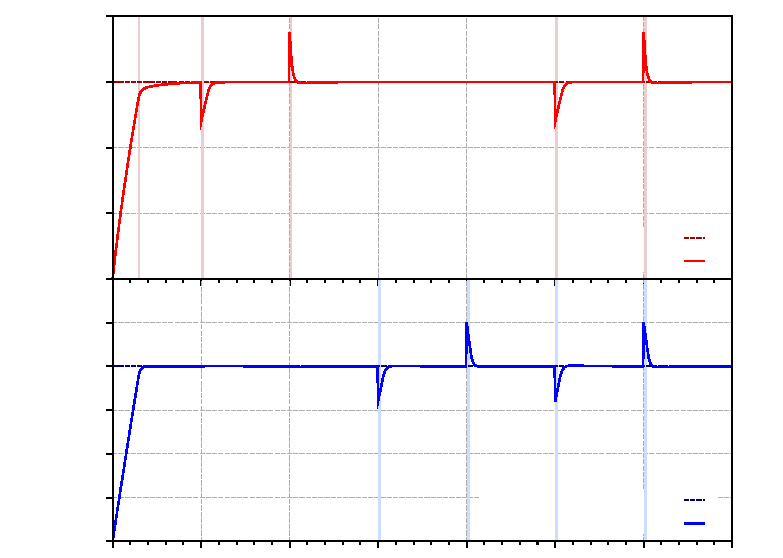
\includegraphics{fsedg}}%
    \gplfronttext
  \end{picture}%
\endgroup
}
\end{figure}
    
\end{frame}

\begin{frame}
    \frametitle{Resultados das simulações}

    Detecção da falha somente no instante de ativação da falha

    \vspace{0.25cm}

    Compensação do controlador (com erro de 20\%) \implica $24 \text{cm} \equiv
    30 \text{cm}$

    \vspace{0.25cm}

    Comportamento semelhante na FSeDO e na FSiVzT

    \vspace{0.25cm}

    Semelhança de comportamento pode dificultar a identificação (proposta 2)

    \vspace{0.25cm}

    Nesse caso a proposta 1 pode apresentar melhores resultados

    \vspace{0.25cm}

    Possibilidade de utilização de {\it flags} para correção do problema

\end{frame}

\begin{frame}
    \frametitle{Resultados das simulações}

\footnotesize Simulação da FSeSR com ruído de distribuição uniforme ($\pm 2\%$):

\begin{figure}[htb]
\footnotesize
\centering
\scalebox{0.68}{% GNUPLOT: LaTeX picture with Postscript
\begingroup
  \makeatletter
  \providecommand\color[2][]{%
    \GenericError{(gnuplot) \space\space\space\@spaces}{%
      Package color not loaded in conjunction with
      terminal option `colourtext'%
    }{See the gnuplot documentation for explanation.%
    }{Either use 'blacktext' in gnuplot or load the package
      color.sty in LaTeX.}%
    \renewcommand\color[2][]{}%
  }%
  \providecommand\includegraphics[2][]{%
    \GenericError{(gnuplot) \space\space\space\@spaces}{%
      Package graphicx or graphics not loaded%
    }{See the gnuplot documentation for explanation.%
    }{The gnuplot epslatex terminal needs graphicx.sty or graphics.sty.}%
    \renewcommand\includegraphics[2][]{}%
  }%
  \providecommand\rotatebox[2]{#2}%
  \@ifundefined{ifGPcolor}{%
    \newif\ifGPcolor
    \GPcolortrue
  }{}%
  \@ifundefined{ifGPblacktext}{%
    \newif\ifGPblacktext
    \GPblacktexttrue
  }{}%
  % define a \g@addto@macro without @ in the name:
  \let\gplgaddtomacro\g@addto@macro
  % define empty templates for all commands taking text:
  \gdef\gplbacktext{}%
  \gdef\gplfronttext{}%
  \makeatother
  \ifGPblacktext
    % no textcolor at all
    \def\colorrgb#1{}%
    \def\colorgray#1{}%
  \else
    % gray or color?
    \ifGPcolor
      \def\colorrgb#1{\color[rgb]{#1}}%
      \def\colorgray#1{\color[gray]{#1}}%
      \expandafter\def\csname LTw\endcsname{\color{white}}%
      \expandafter\def\csname LTb\endcsname{\color{black}}%
      \expandafter\def\csname LTa\endcsname{\color{black}}%
      \expandafter\def\csname LT0\endcsname{\color[rgb]{1,0,0}}%
      \expandafter\def\csname LT1\endcsname{\color[rgb]{0,1,0}}%
      \expandafter\def\csname LT2\endcsname{\color[rgb]{0,0,1}}%
      \expandafter\def\csname LT3\endcsname{\color[rgb]{1,0,1}}%
      \expandafter\def\csname LT4\endcsname{\color[rgb]{0,1,1}}%
      \expandafter\def\csname LT5\endcsname{\color[rgb]{1,1,0}}%
      \expandafter\def\csname LT6\endcsname{\color[rgb]{0,0,0}}%
      \expandafter\def\csname LT7\endcsname{\color[rgb]{1,0.3,0}}%
      \expandafter\def\csname LT8\endcsname{\color[rgb]{0.5,0.5,0.5}}%
    \else
      % gray
      \def\colorrgb#1{\color{black}}%
      \def\colorgray#1{\color[gray]{#1}}%
      \expandafter\def\csname LTw\endcsname{\color{white}}%
      \expandafter\def\csname LTb\endcsname{\color{black}}%
      \expandafter\def\csname LTa\endcsname{\color{black}}%
      \expandafter\def\csname LT0\endcsname{\color{black}}%
      \expandafter\def\csname LT1\endcsname{\color{black}}%
      \expandafter\def\csname LT2\endcsname{\color{black}}%
      \expandafter\def\csname LT3\endcsname{\color{black}}%
      \expandafter\def\csname LT4\endcsname{\color{black}}%
      \expandafter\def\csname LT5\endcsname{\color{black}}%
      \expandafter\def\csname LT6\endcsname{\color{black}}%
      \expandafter\def\csname LT7\endcsname{\color{black}}%
      \expandafter\def\csname LT8\endcsname{\color{black}}%
    \fi
  \fi
  \setlength{\unitlength}{0.0500bp}%
  \begin{picture}(7200.00,5040.00)%
    \gplgaddtomacro\gplbacktext{%
      \csname LTb\endcsname%
      \put(726,3150){\makebox(0,0)[r]{\strut{} 5}}%
      \csname LTb\endcsname%
      \put(726,3780){\makebox(0,0)[r]{\strut{} 10}}%
      \csname LTb\endcsname%
      \put(726,4409){\makebox(0,0)[r]{\strut{} 15}}%
      \csname LTb\endcsname%
      \put(726,5039){\makebox(0,0)[r]{\strut{} 20}}%
      \csname LTb\endcsname%
      \put(921,2237){\makebox(0,0){\strut{}}}%
      \csname LTb\endcsname%
      \put(1771,2237){\makebox(0,0){\strut{}}}%
      \csname LTb\endcsname%
      \put(2620,2237){\makebox(0,0){\strut{}}}%
      \csname LTb\endcsname%
      \put(3470,2237){\makebox(0,0){\strut{}}}%
      \csname LTb\endcsname%
      \put(4320,2237){\makebox(0,0){\strut{}}}%
      \csname LTb\endcsname%
      \put(5170,2237){\makebox(0,0){\strut{}}}%
      \csname LTb\endcsname%
      \put(6019,2237){\makebox(0,0){\strut{}}}%
      \csname LTb\endcsname%
      \put(6869,2237){\makebox(0,0){\strut{}}}%
      \put(352,3779){\rotatebox{-270}{\makebox(0,0){\strut{}Nível [cm]}}}%
    }%
    \gplgaddtomacro\gplfronttext{%
      \csname LTb\endcsname%
      \put(6278,2913){\makebox(0,0)[r]{\strut{}Ref. $T_1$}}%
      \csname LTb\endcsname%
      \put(6278,2693){\makebox(0,0)[r]{\strut{}Saída $T_1$}}%
    }%
    \gplgaddtomacro\gplbacktext{%
      \csname LTb\endcsname%
      \put(726,0){\makebox(0,0)[r]{\strut{} 0}}%
      \csname LTb\endcsname%
      \put(726,504){\makebox(0,0)[r]{\strut{} 5}}%
      \csname LTb\endcsname%
      \put(726,1008){\makebox(0,0)[r]{\strut{} 10}}%
      \csname LTb\endcsname%
      \put(726,1512){\makebox(0,0)[r]{\strut{} 15}}%
      \csname LTb\endcsname%
      \put(726,2016){\makebox(0,0)[r]{\strut{} 20}}%
      \csname LTb\endcsname%
      \put(726,2520){\makebox(0,0)[r]{\strut{} 25}}%
      \csname LTb\endcsname%
      \put(921,-283){\makebox(0,0){\strut{}0}}%
      \csname LTb\endcsname%
      \put(1771,-283){\makebox(0,0){\strut{}15}}%
      \csname LTb\endcsname%
      \put(2620,-283){\makebox(0,0){\strut{}30}}%
      \csname LTb\endcsname%
      \put(3470,-283){\makebox(0,0){\strut{}45}}%
      \csname LTb\endcsname%
      \put(4320,-283){\makebox(0,0){\strut{}60}}%
      \csname LTb\endcsname%
      \put(5170,-283){\makebox(0,0){\strut{}75}}%
      \csname LTb\endcsname%
      \put(6019,-283){\makebox(0,0){\strut{}90}}%
      \csname LTb\endcsname%
      \put(6869,-283){\makebox(0,0){\strut{}105}}%
      \put(352,1260){\rotatebox{-270}{\makebox(0,0){\strut{}Nível [cm]}}}%
      \put(3895,-613){\makebox(0,0){\strut{}Tempo [s]}}%
    }%
    \gplgaddtomacro\gplfronttext{%
      \csname LTb\endcsname%
      \put(6278,393){\makebox(0,0)[r]{\strut{}Ref. $T_2$}}%
      \csname LTb\endcsname%
      \put(6278,173){\makebox(0,0)[r]{\strut{}Saída $T_2$}}%
    }%
    \gplbacktext
    \put(0,0){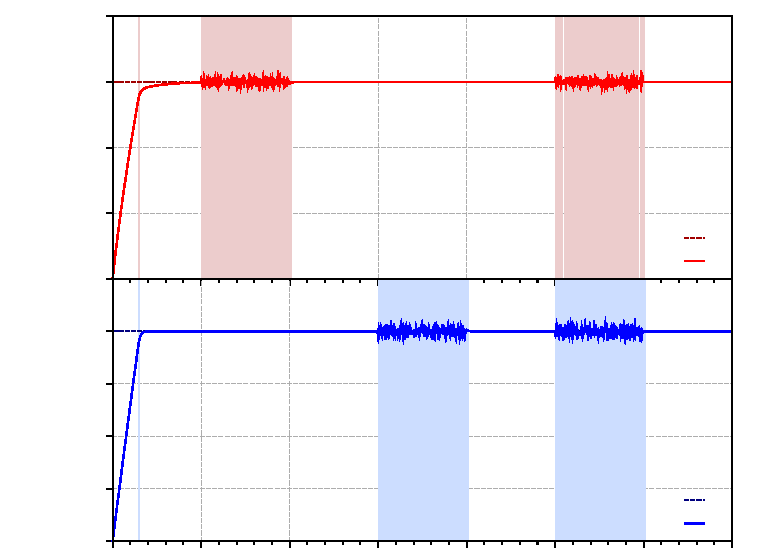
\includegraphics{fsesr}}%
    \gplfronttext
  \end{picture}%
\endgroup
}
\end{figure}
    
\end{frame}

\begin{frame}
    \frametitle{Resultados das simulações}

    Bons resultados \implica poucos erros

    \vspace{0.25cm}

    Exceto pelas FASR e FSiVrGMP, todas as demais falhas se comportaram de
    maneira semelhante \implica facilmente detectadas

    \vspace{0.25cm}

    FASR:

\begin{itemize}
    \item Resultados $T_1$ \alert{\Checkmark}
    \item Resultados $T_2$ \alert{\XSolidBrush}
\end{itemize}

    FSiVrGMP:

\begin{itemize}
    \item Não consegue identificar falha somente em $T_1$ (intervalo 15-30s)
\end{itemize}

\end{frame}

\begin{frame}
    \frametitle{Resultados das simulações}

\footnotesize Simulação da FASR com ruído de distribuição uniforme ($\pm 2\%$):

\begin{figure}[htb] 
\footnotesize 
\centering 
\scalebox{0.68}{% GNUPLOT: LaTeX picture with Postscript
\begingroup
  \makeatletter
  \providecommand\color[2][]{%
    \GenericError{(gnuplot) \space\space\space\@spaces}{%
      Package color not loaded in conjunction with
      terminal option `colourtext'%
    }{See the gnuplot documentation for explanation.%
    }{Either use 'blacktext' in gnuplot or load the package
      color.sty in LaTeX.}%
    \renewcommand\color[2][]{}%
  }%
  \providecommand\includegraphics[2][]{%
    \GenericError{(gnuplot) \space\space\space\@spaces}{%
      Package graphicx or graphics not loaded%
    }{See the gnuplot documentation for explanation.%
    }{The gnuplot epslatex terminal needs graphicx.sty or graphics.sty.}%
    \renewcommand\includegraphics[2][]{}%
  }%
  \providecommand\rotatebox[2]{#2}%
  \@ifundefined{ifGPcolor}{%
    \newif\ifGPcolor
    \GPcolortrue
  }{}%
  \@ifundefined{ifGPblacktext}{%
    \newif\ifGPblacktext
    \GPblacktexttrue
  }{}%
  % define a \g@addto@macro without @ in the name:
  \let\gplgaddtomacro\g@addto@macro
  % define empty templates for all commands taking text:
  \gdef\gplbacktext{}%
  \gdef\gplfronttext{}%
  \makeatother
  \ifGPblacktext
    % no textcolor at all
    \def\colorrgb#1{}%
    \def\colorgray#1{}%
  \else
    % gray or color?
    \ifGPcolor
      \def\colorrgb#1{\color[rgb]{#1}}%
      \def\colorgray#1{\color[gray]{#1}}%
      \expandafter\def\csname LTw\endcsname{\color{white}}%
      \expandafter\def\csname LTb\endcsname{\color{black}}%
      \expandafter\def\csname LTa\endcsname{\color{black}}%
      \expandafter\def\csname LT0\endcsname{\color[rgb]{1,0,0}}%
      \expandafter\def\csname LT1\endcsname{\color[rgb]{0,1,0}}%
      \expandafter\def\csname LT2\endcsname{\color[rgb]{0,0,1}}%
      \expandafter\def\csname LT3\endcsname{\color[rgb]{1,0,1}}%
      \expandafter\def\csname LT4\endcsname{\color[rgb]{0,1,1}}%
      \expandafter\def\csname LT5\endcsname{\color[rgb]{1,1,0}}%
      \expandafter\def\csname LT6\endcsname{\color[rgb]{0,0,0}}%
      \expandafter\def\csname LT7\endcsname{\color[rgb]{1,0.3,0}}%
      \expandafter\def\csname LT8\endcsname{\color[rgb]{0.5,0.5,0.5}}%
    \else
      % gray
      \def\colorrgb#1{\color{black}}%
      \def\colorgray#1{\color[gray]{#1}}%
      \expandafter\def\csname LTw\endcsname{\color{white}}%
      \expandafter\def\csname LTb\endcsname{\color{black}}%
      \expandafter\def\csname LTa\endcsname{\color{black}}%
      \expandafter\def\csname LT0\endcsname{\color{black}}%
      \expandafter\def\csname LT1\endcsname{\color{black}}%
      \expandafter\def\csname LT2\endcsname{\color{black}}%
      \expandafter\def\csname LT3\endcsname{\color{black}}%
      \expandafter\def\csname LT4\endcsname{\color{black}}%
      \expandafter\def\csname LT5\endcsname{\color{black}}%
      \expandafter\def\csname LT6\endcsname{\color{black}}%
      \expandafter\def\csname LT7\endcsname{\color{black}}%
      \expandafter\def\csname LT8\endcsname{\color{black}}%
    \fi
  \fi
  \setlength{\unitlength}{0.0500bp}%
  \begin{picture}(7200.00,5040.00)%
    \gplgaddtomacro\gplbacktext{%
      \csname LTb\endcsname%
      \put(726,3150){\makebox(0,0)[r]{\strut{} 5}}%
      \csname LTb\endcsname%
      \put(726,3780){\makebox(0,0)[r]{\strut{} 10}}%
      \csname LTb\endcsname%
      \put(726,4409){\makebox(0,0)[r]{\strut{} 15}}%
      \csname LTb\endcsname%
      \put(726,5039){\makebox(0,0)[r]{\strut{} 20}}%
      \csname LTb\endcsname%
      \put(921,2237){\makebox(0,0){\strut{}}}%
      \csname LTb\endcsname%
      \put(1771,2237){\makebox(0,0){\strut{}}}%
      \csname LTb\endcsname%
      \put(2620,2237){\makebox(0,0){\strut{}}}%
      \csname LTb\endcsname%
      \put(3470,2237){\makebox(0,0){\strut{}}}%
      \csname LTb\endcsname%
      \put(4320,2237){\makebox(0,0){\strut{}}}%
      \csname LTb\endcsname%
      \put(5170,2237){\makebox(0,0){\strut{}}}%
      \csname LTb\endcsname%
      \put(6019,2237){\makebox(0,0){\strut{}}}%
      \csname LTb\endcsname%
      \put(6869,2237){\makebox(0,0){\strut{}}}%
      \put(352,3779){\rotatebox{-270}{\makebox(0,0){\strut{}Level [cm]}}}%
    }%
    \gplgaddtomacro\gplfronttext{%
      \csname LTb\endcsname%
      \put(6278,2913){\makebox(0,0)[r]{\strut{}Setpoint $T_1$}}%
      \csname LTb\endcsname%
      \put(6278,2693){\makebox(0,0)[r]{\strut{}Output $T_1$}}%
    }%
    \gplgaddtomacro\gplbacktext{%
      \csname LTb\endcsname%
      \put(726,0){\makebox(0,0)[r]{\strut{} 0}}%
      \csname LTb\endcsname%
      \put(726,840){\makebox(0,0)[r]{\strut{} 10}}%
      \csname LTb\endcsname%
      \put(726,1680){\makebox(0,0)[r]{\strut{} 20}}%
      \csname LTb\endcsname%
      \put(726,2520){\makebox(0,0)[r]{\strut{} 30}}%
      \csname LTb\endcsname%
      \put(921,-283){\makebox(0,0){\strut{}0}}%
      \csname LTb\endcsname%
      \put(1771,-283){\makebox(0,0){\strut{}15}}%
      \csname LTb\endcsname%
      \put(2620,-283){\makebox(0,0){\strut{}30}}%
      \csname LTb\endcsname%
      \put(3470,-283){\makebox(0,0){\strut{}45}}%
      \csname LTb\endcsname%
      \put(4320,-283){\makebox(0,0){\strut{}60}}%
      \csname LTb\endcsname%
      \put(5170,-283){\makebox(0,0){\strut{}75}}%
      \csname LTb\endcsname%
      \put(6019,-283){\makebox(0,0){\strut{}90}}%
      \csname LTb\endcsname%
      \put(6869,-283){\makebox(0,0){\strut{}105}}%
      \put(352,1260){\rotatebox{-270}{\makebox(0,0){\strut{}Level [cm]}}}%
      \put(3895,-613){\makebox(0,0){\strut{}Time [s]}}%
    }%
    \gplgaddtomacro\gplfronttext{%
      \csname LTb\endcsname%
      \put(6278,393){\makebox(0,0)[r]{\strut{}Setpoint $T_2$}}%
      \csname LTb\endcsname%
      \put(6278,173){\makebox(0,0)[r]{\strut{}Output $T_2$}}%
    }%
    \gplbacktext
    \put(0,0){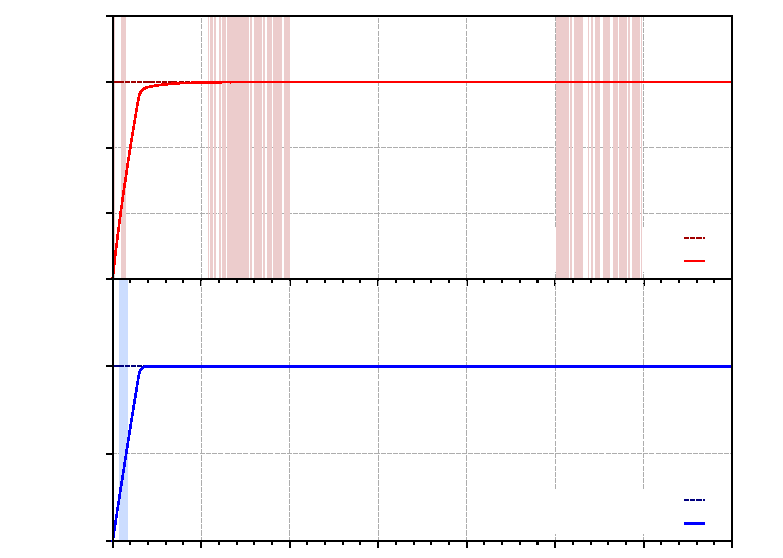
\includegraphics{fasr}}%
    \gplfronttext
  \end{picture}%
\endgroup
}
\end{figure}
    
\end{frame}

\begin{frame}
    \frametitle{Resultados das simulações}

\footnotesize Simulação da FSiVrGMP com o ganho reduzido a 90\% do valor
original:

\begin{figure}[htb] 
\footnotesize 
\centering 
\scalebox{0.68}{% GNUPLOT: LaTeX picture with Postscript
\begingroup
  \makeatletter
  \providecommand\color[2][]{%
    \GenericError{(gnuplot) \space\space\space\@spaces}{%
      Package color not loaded in conjunction with
      terminal option `colourtext'%
    }{See the gnuplot documentation for explanation.%
    }{Either use 'blacktext' in gnuplot or load the package
      color.sty in LaTeX.}%
    \renewcommand\color[2][]{}%
  }%
  \providecommand\includegraphics[2][]{%
    \GenericError{(gnuplot) \space\space\space\@spaces}{%
      Package graphicx or graphics not loaded%
    }{See the gnuplot documentation for explanation.%
    }{The gnuplot epslatex terminal needs graphicx.sty or graphics.sty.}%
    \renewcommand\includegraphics[2][]{}%
  }%
  \providecommand\rotatebox[2]{#2}%
  \@ifundefined{ifGPcolor}{%
    \newif\ifGPcolor
    \GPcolortrue
  }{}%
  \@ifundefined{ifGPblacktext}{%
    \newif\ifGPblacktext
    \GPblacktexttrue
  }{}%
  % define a \g@addto@macro without @ in the name:
  \let\gplgaddtomacro\g@addto@macro
  % define empty templates for all commands taking text:
  \gdef\gplbacktext{}%
  \gdef\gplfronttext{}%
  \makeatother
  \ifGPblacktext
    % no textcolor at all
    \def\colorrgb#1{}%
    \def\colorgray#1{}%
  \else
    % gray or color?
    \ifGPcolor
      \def\colorrgb#1{\color[rgb]{#1}}%
      \def\colorgray#1{\color[gray]{#1}}%
      \expandafter\def\csname LTw\endcsname{\color{white}}%
      \expandafter\def\csname LTb\endcsname{\color{black}}%
      \expandafter\def\csname LTa\endcsname{\color{black}}%
      \expandafter\def\csname LT0\endcsname{\color[rgb]{1,0,0}}%
      \expandafter\def\csname LT1\endcsname{\color[rgb]{0,1,0}}%
      \expandafter\def\csname LT2\endcsname{\color[rgb]{0,0,1}}%
      \expandafter\def\csname LT3\endcsname{\color[rgb]{1,0,1}}%
      \expandafter\def\csname LT4\endcsname{\color[rgb]{0,1,1}}%
      \expandafter\def\csname LT5\endcsname{\color[rgb]{1,1,0}}%
      \expandafter\def\csname LT6\endcsname{\color[rgb]{0,0,0}}%
      \expandafter\def\csname LT7\endcsname{\color[rgb]{1,0.3,0}}%
      \expandafter\def\csname LT8\endcsname{\color[rgb]{0.5,0.5,0.5}}%
    \else
      % gray
      \def\colorrgb#1{\color{black}}%
      \def\colorgray#1{\color[gray]{#1}}%
      \expandafter\def\csname LTw\endcsname{\color{white}}%
      \expandafter\def\csname LTb\endcsname{\color{black}}%
      \expandafter\def\csname LTa\endcsname{\color{black}}%
      \expandafter\def\csname LT0\endcsname{\color{black}}%
      \expandafter\def\csname LT1\endcsname{\color{black}}%
      \expandafter\def\csname LT2\endcsname{\color{black}}%
      \expandafter\def\csname LT3\endcsname{\color{black}}%
      \expandafter\def\csname LT4\endcsname{\color{black}}%
      \expandafter\def\csname LT5\endcsname{\color{black}}%
      \expandafter\def\csname LT6\endcsname{\color{black}}%
      \expandafter\def\csname LT7\endcsname{\color{black}}%
      \expandafter\def\csname LT8\endcsname{\color{black}}%
    \fi
  \fi
  \setlength{\unitlength}{0.0500bp}%
  \begin{picture}(7200.00,5040.00)%
    \gplgaddtomacro\gplbacktext{%
      \csname LTb\endcsname%
      \put(726,3150){\makebox(0,0)[r]{\strut{} 5}}%
      \csname LTb\endcsname%
      \put(726,3780){\makebox(0,0)[r]{\strut{} 10}}%
      \csname LTb\endcsname%
      \put(726,4409){\makebox(0,0)[r]{\strut{} 15}}%
      \csname LTb\endcsname%
      \put(726,5039){\makebox(0,0)[r]{\strut{} 20}}%
      \csname LTb\endcsname%
      \put(921,2237){\makebox(0,0){\strut{}}}%
      \csname LTb\endcsname%
      \put(1771,2237){\makebox(0,0){\strut{}}}%
      \csname LTb\endcsname%
      \put(2620,2237){\makebox(0,0){\strut{}}}%
      \csname LTb\endcsname%
      \put(3470,2237){\makebox(0,0){\strut{}}}%
      \csname LTb\endcsname%
      \put(4320,2237){\makebox(0,0){\strut{}}}%
      \csname LTb\endcsname%
      \put(5170,2237){\makebox(0,0){\strut{}}}%
      \csname LTb\endcsname%
      \put(6019,2237){\makebox(0,0){\strut{}}}%
      \csname LTb\endcsname%
      \put(6869,2237){\makebox(0,0){\strut{}}}%
      \put(352,3779){\rotatebox{-270}{\makebox(0,0){\strut{}Nível [cm]}}}%
    }%
    \gplgaddtomacro\gplfronttext{%
      \csname LTb\endcsname%
      \put(6278,2913){\makebox(0,0)[r]{\strut{}Ref. $T_1$}}%
      \csname LTb\endcsname%
      \put(6278,2693){\makebox(0,0)[r]{\strut{}Saída $T_1$}}%
    }%
    \gplgaddtomacro\gplbacktext{%
      \csname LTb\endcsname%
      \put(726,0){\makebox(0,0)[r]{\strut{} 0}}%
      \csname LTb\endcsname%
      \put(726,840){\makebox(0,0)[r]{\strut{} 10}}%
      \csname LTb\endcsname%
      \put(726,1680){\makebox(0,0)[r]{\strut{} 20}}%
      \csname LTb\endcsname%
      \put(726,2520){\makebox(0,0)[r]{\strut{} 30}}%
      \csname LTb\endcsname%
      \put(921,-283){\makebox(0,0){\strut{}0}}%
      \csname LTb\endcsname%
      \put(1771,-283){\makebox(0,0){\strut{}15}}%
      \csname LTb\endcsname%
      \put(2620,-283){\makebox(0,0){\strut{}30}}%
      \csname LTb\endcsname%
      \put(3470,-283){\makebox(0,0){\strut{}45}}%
      \csname LTb\endcsname%
      \put(4320,-283){\makebox(0,0){\strut{}60}}%
      \csname LTb\endcsname%
      \put(5170,-283){\makebox(0,0){\strut{}75}}%
      \csname LTb\endcsname%
      \put(6019,-283){\makebox(0,0){\strut{}90}}%
      \csname LTb\endcsname%
      \put(6869,-283){\makebox(0,0){\strut{}105}}%
      \put(352,1260){\rotatebox{-270}{\makebox(0,0){\strut{}Nível [cm]}}}%
      \put(3895,-613){\makebox(0,0){\strut{}Tempo [s]}}%
    }%
    \gplgaddtomacro\gplfronttext{%
      \csname LTb\endcsname%
      \put(6278,393){\makebox(0,0)[r]{\strut{}Ref. $T_2$}}%
      \csname LTb\endcsname%
      \put(6278,173){\makebox(0,0)[r]{\strut{}Saída $T_2$}}%
    }%
    \gplbacktext
    \put(0,0){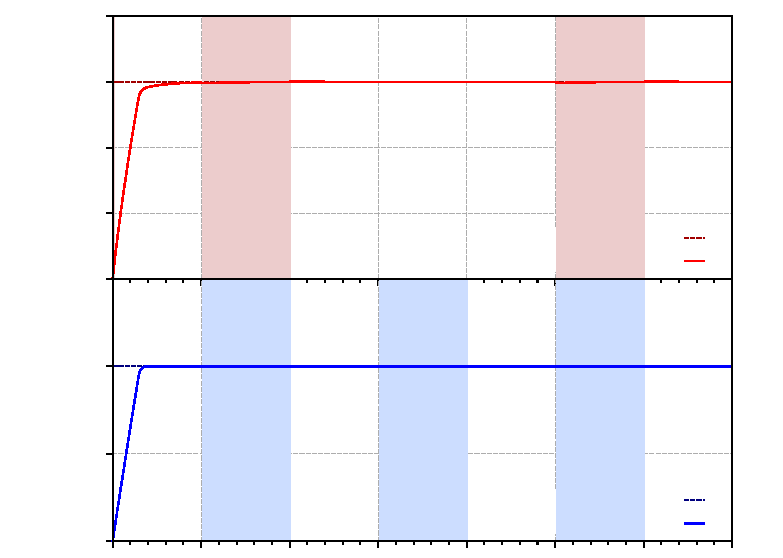
\includegraphics{fsivrgmp}}%
    \gplfronttext
  \end{picture}%
\endgroup
}
\end{figure}
    
\end{frame}

% Conclusões -------------------------------------------------------------------
\section{Conclusões}
% ------------------------------------------------------------------------------
\subsection*{Conclusões}
\begin{frame}
    \frametitle{Conclusões}

    Proposta do trabalho: fornecer um sistema de DDF para um sistema de tanques
    acoplados

\begin{itemize}
    \item Das 13 falhas testadas, 8 foram identificadas com facilidade
    \item 3 tiveram desempenho satisfatório (correção do problema com {\it
          flags})
    \item Outros 2 casos o sistema não conseguiu detectar corretamente 
    \begin{itemize}
        \item Detecção correta somente para $T_1$
    \end{itemize}
\end{itemize}

    Desempenho geral satisfatório: detecção correta de 85\% das falhas propostas

    \vspace{0.25cm}

    Utilização de RNAs (PMC, NNARX) mostrou-se eficiente

\end{frame}

% ------------------------------------------------------------------------------
\subsection{Perspectivas}
\begin{frame}
    \frametitle{Perspectivas}

    Atividades a serem realizadas:

\begin{itemize}
    \item Simulação de falhas (individual -- proposta 1)
    \item Combinações de falhas (proposta 1 e 2)
    \item RNAs agindo em paralelo (proposta 2)
\end{itemize}

    Possíveis trabalhos futuros:
\begin{itemize}
    \item Adição das redes neurais ao sistema desenvolvido em C++
    \begin{itemize}
        \item Possibilidade de observação das falhas em tempo de execução
        \item Visualização dos alarmes por parte do operador
    \end{itemize}
    \item Acoplamento à um Sistema de Controle Tolerante a Falhas (SCTF) -- Não
          é o escopo deste trabalho
    \begin{itemize}
        \item Reconfiguração dos controladores ou mudança das estratégias de
              controle
    \end{itemize}
\end{itemize}

\end{frame}

% ------------------------------------------------------------------------------
\subsection{Cronograma de atividades}
\begin{frame}
    \frametitle{Cronograma de atividades}

    Atividades executadas/pendentes:

\begin{figure}[htb]
\centering
    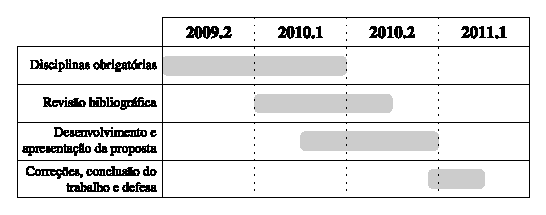
\includegraphics[width=0.85\textwidth]{imgs/conclusoes/eps/cronograma}
\end{figure}
    
\end{frame}

% Dúvidas ----------------------------------------------------------------------
\section*{Dúvidas}
% ------------------------------------------------------------------------------
\subsection*{Dúvidas}
\begin{frame}
    \frametitle{Dúvidas}

    \Large Dúvidas?
\end{frame}

\end{document}
